%This is the fourth chapter of the dissertation

%The following command starts your chapter. If you want different titles used in your ToC and at the top of the page throughout the chapter, you can specify those values here. Since Columbia doesn't want extra information in the headers and footers, the "Top of Page Title" value won't actually appear.

\pagestyle{cu}
\graphicspath{{./Chapter4/images/}}

\chapter[Measuring the Low Energy Light and Charge Yield of Nuclear Recoils in Liquid Xenon][Measuring the Low Energy Light and Charge Yield of Nuclear Recoils in Liquid Xenon]{Measuring the Low Energy Light and Charge Yield of Nuclear Recoils in Liquid Xenon}
\label{chap:nerix}

%As was discussed in the second and third chapter of this work, understanding the response of liquid xenon to nuclear recoils is very important for the dark matter search as many candidates, including WIMPs, are expected to interact with atomic nuclei.  Liquid xenon detectors continue to grow in size yet this only makes their calibration, specifically with regards to nuclear recoils, increasingly difficult.  

As was discussed in the previous chapters, dual-phase liquid xenon TPCs lead the search for WIMPs.  These detectors continue to grow in size and reduce their background making them increasingly more sensitive to dark matter.  As mentioned in the previous chapter, XENON1T is the largest and most sensitive of these detectors with a total mass of 3,200 kg of liquid xenon \cite{aprile2017first}.  Since WIMPs are expected to interact primarily with atomic nuclei and the differential scattering rate of WIMPs and Standard Model particles are generally expected to increase with decreasing interaction energy, it is crucial to understand the properties of nuclear recoils in LXe down to the few keV energy scale.  

While larger detector sizes (in the form of larger fiducial volumes) make WIMP searches more and more sensitive, they do come with a drawback: calibrations, especially calibrations with external sources, becoming significantly more difficult.   However, understanding the signal output by a LXe TPC can essentially be broken down into two steps: the actual light and charge production and the detector physics.  While the detector physics is unique for each detector used and therefore must be measured for each one, the light and charge production mechanisms are only unique to the medium.  Therefore, if we can effectively decouple the two steps, we can measure the light and charge production mechanism in a detector optimized for calibrations and use it in other detectors.  

As LXe detectors have scaled in size, several of these optimized detectors have been built for exactly this purpose: to measure the light and charge production of liquid xenon to electronic and nuclear recoils.  While each of these detectors was slightly different and designed for a specific purpose, they shared the same relatively simple operating procedure: measure the light and charge produced from an interaction of a known type (electronic or nuclear recoil) and energy.  The neriX (Nuclear and Electronic Recoils in xenon) detector at Columbia University is one of these optimized detectors and has already successfully provided the most precise measurements of the light and charge yield (the number of photons and electrons produced per unit energy) of electronic recoils in liquid xenon at multiple electric fields.  

While several measurements of the response of liquid xenon to nuclear recoils have been made, most measure only the light yield or charge yield.  Two particular calibrations \cite{aprile2006simultaneous, manzur2010scintillation} measure both the light and charge yield but do not capture the potential correlation of the yields.  Without examining both light and charge simultaneously, it is impossible to fully understand the fundamental processes that occur in LXe to produce these signals.  Additionally, only the two simultaneous studies \cite{aprile2006simultaneous, manzur2010scintillation} have systematically measured the effect of an electric field on the light and charge yield.  Unlike in the case of electronic recoils, these measurements found that the light and charge yield of nuclear recoils in liquid xenon change very little, if at all, with an applied electric field.  However, additional measurements are necessary since it is expected that the recombination of electrons and ions produced in the interaction is energy dependent as well as field dependent \cite{thomas1987recombination} and both measurements cannot make conclusive statements below $\sim 45$~keV.  In this chapter the results of a new measurement of both the light and charge yield of nuclear recoils from 74 keV down to 3~keV at three electric fields using the fixed-angle scattering method are presented.  Also, for the first time, a simulation of the light and charge production process in liquid xenon is used for the parameter estimation, which takes into account the correlation between the light and charge signals.

%In this chapter, we will discuss the measurement of the light and charge yield of low energy nuclear recoils in liquid xenon using the neriX detector at Columbia University.

\section{Experimental Setup}
\label{sec:nerix_expt_setup}

In chapter three, we discussed the nuclear recoil calibration of XENON1T.  In this calibration, an americium-beryllium (AmBe) source was used to irradiate the liquid xenon inside of the detector with MeV energy neutrons.  Simulation is performed to determine the energy spectrum of single scatters in the detectors but, for the most part, the spectrum is defined by the relative cross-section of elastic scatters at different energies ultimately resulting in an exponentially falling energy spectrum as seen in \figref{fig:xe1t_nr_energy_spec}.  In this calibration setup, the energy of each individual event is unknown and we are using the entire energy spectrum to match our data.  While this can be an effective way to measure the response of liquid xenon to nuclear recoils, it proves to be very difficult in practice with such a featureless energy spectrum.  This type of measurement where one compares an energy spectrum to data is typically referred to as an \textit{indirect} measurement and has been used successfully to measure the light and charge production process of electronic and nuclear recoils \cite{aprile2013response, akerib2016tritium, aprile2017tritium}.

Measurements in neriX and other smaller, calibration optimized detectors follow a different approach.  A monoenergetic source is used to irradiate the detector where the incoming particle will scatter a single time before scattering into a secondary detector.  For electronic recoils, the secondary detector can be a high-purity germanium detector or sodium-iodide detector with an excellent energy resolution.  When this is the case, assuming the incoming radiation did not scatter with other materials around the detector, the energy of the interaction is known very precisely.  Unfortunately when measuring the response of liquid xenon to nuclear recoils in these detectors, no equivalent secondary detectors exist that will precisely measure the energy of the incoming neutron.  Instead we can use the position of the secondary detector as a proxy for the energy since the energy transferred to a xenon nucleus by a neutron is completely determined by the scattering angle.  This relationship between the energy of the recoiling nucleus and the angle is shown for non-relativistic neutron energies in \eqnref{eqn:nerix_energy_scattering_angle} where $m_n$ is the mass of the neutron, $m_{\textrm{Xe}}$ is the mass of the xenon nucleus, $E_r$ is the energy of the recoiling nucleus, $E_n$ is the energy of the incoming neutron, and $\theta$ is the scattering angle \cite{knoll2010radiation}.

\begin{equation}
        \label{eqn:nerix_energy_scattering_angle}
        E_r \approx E_n \frac{2 m_n m_{\textrm{Xe}}}{(m_n + m_{\textrm{Xe}})^2}(1 - \textrm{cos} \, \theta)
\end{equation}

A schematic of the experimental setup for neriX using this \textit{fixed-angle scatttering} technique is shown in \figref{fig:nerix_expt_schematic}.  The neutron source in this measurement was a \ce{^2H}$(d, n)$\ce{^3He} generator provided by the Schlumberger Princeton Technology Center which produces 2.45 MeV neutrons at an angle of $\frac{\pi}{2}$.  The secondary detectors used were Eljen Technologies M510 detectors filled with the EJ301 liquid scintillator, chosen for their excellent pulse shape discrimination \cite{ej301_manual}.  


\begin{figure}[t]
        \centering
	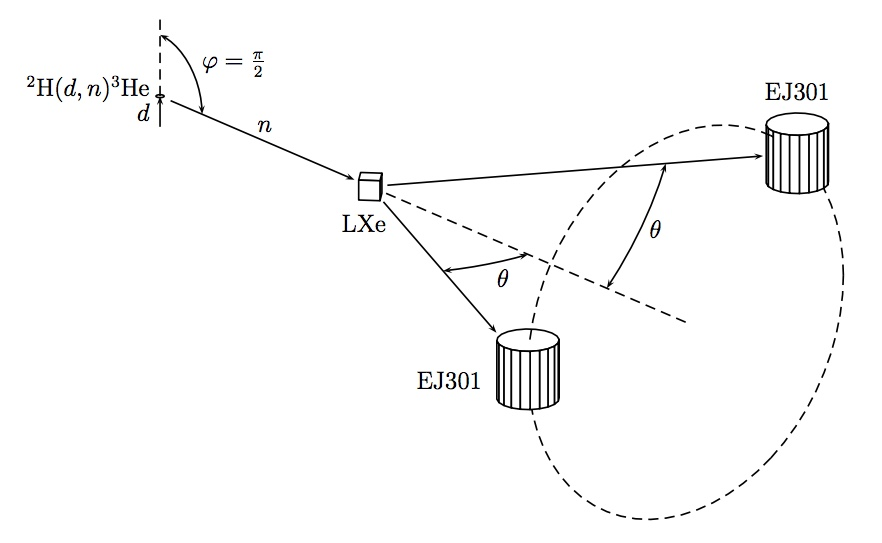
\includegraphics[width=0.9\textwidth]{nerix_expt_schematic}
	\caption{A schematic for the experimental setup used in this measurement of the light and charge yields for nuclear recoils.  2.45 MeV neutrons are produced at an angle of $\frac{\pi}{2}$ in the neutron generator.  Some of these neutrons scatter a single time in the liquid xenon and then deposit some of their energy in the M510 detectors, filled with EJ301 liquid scintillator, for discrimination versus background.  Image Credit: \citeref{plante2011new}.}
	\label{fig:nerix_expt_schematic}
\end{figure}


\begin{figure}[bt]
        \centering
	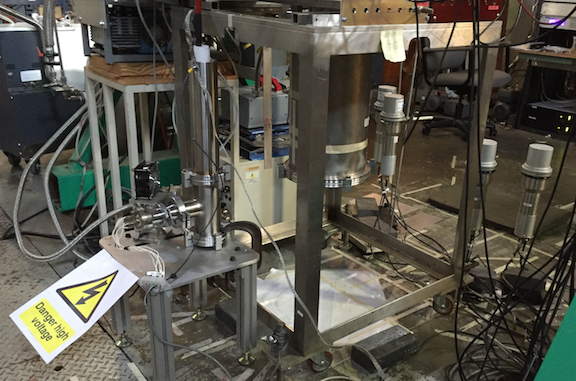
\includegraphics[width=0.9\textwidth]{nerix_experimental_setup}
	\caption{A photo of the fixed-angle scattering setup with the neriX detector.  On the left is our neutron generator inside of its stainless steel case.  In the center is the outer portion of the cryostat and on the right are four of the M510 liquid scintillator detectors.}
	\label{fig:nerix_experimental_setup}
\end{figure}



\subsection{neriX Detector}

In this section we will discuss the neriX detector.  neriX was specifically designed to minimize the amount of inactive xenon and materials surrounding the TPC to minimize undetectable energy depositions and with electronics such that it can systematically scan electric fields ranging from approximately 0.15 V/cm to 2.5 kV/cm in the LXe.  These features make neriX an ideal detector for measuring the low-energy response of electronic and nuclear recoils at electric fields relevant to the dark matter search.

For more details on the design and construction of neriX, please refer to chapters four and five of \citeref{goetzke2015low}.

\subsubsection{TPC}

The neriX TPC (shown in \figref{fig:nerix_tpc_labeled}), like XENON1T, was also constructed with PTFE (teflon).  The teflon pieces in neriX are stackable and compressed by stainless steel springs.  The TPC at liquid xenon temperature has an inner diameter of 43 mm.  neriX also included four stainless steel hexagonal meshes and a single field shaping ring to control the electric fields inside of the TPC.  The cathode (used to produce the high voltage for the drift field inside the liquid xenon), the gate (kept at ground near the liquid surface), and the anode (used to extract electrons from the liquid surface and into the gas) were each made of  125 $\mu$m thick wires and 3 mm pitch (distance between parallel wire segments).  A photo of the gate mesh from above is shown in \figref{fig:nerix_tpc_mesh}.  The final mesh was a screening mesh (labeled the ``bottom grid'' in \figref{fig:nerix_tpc_labeled}) used to shield the bottom PMT and was also made with a 3 mm pitch but with 25 $\mu$m thick wires (to reduce its surface area).  The field shaping ring is simply a copper coaxial wire embedded in the teflon wall of the TPC 7 mm above the cathode.  The location of the shaping ring was to maximize uniformity of the drift field at an electric field of 1 kV/cm.  The distance between the cathode and the gate mesh, the maximum drift distance of electrons in the TPC, was 23.4 mm.


\begin{figure}[t]
        \centering
	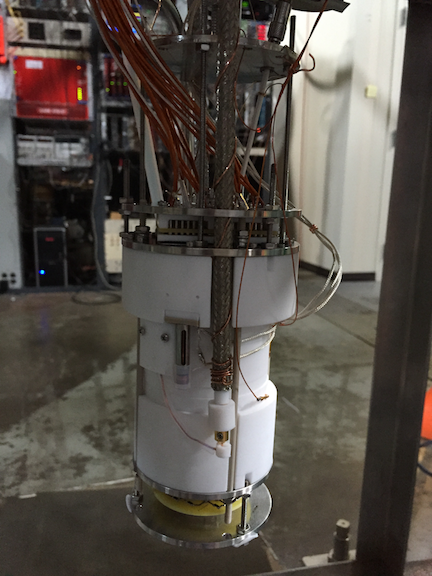
\includegraphics[width=0.50\textwidth]{nerix_tpc_anode}
	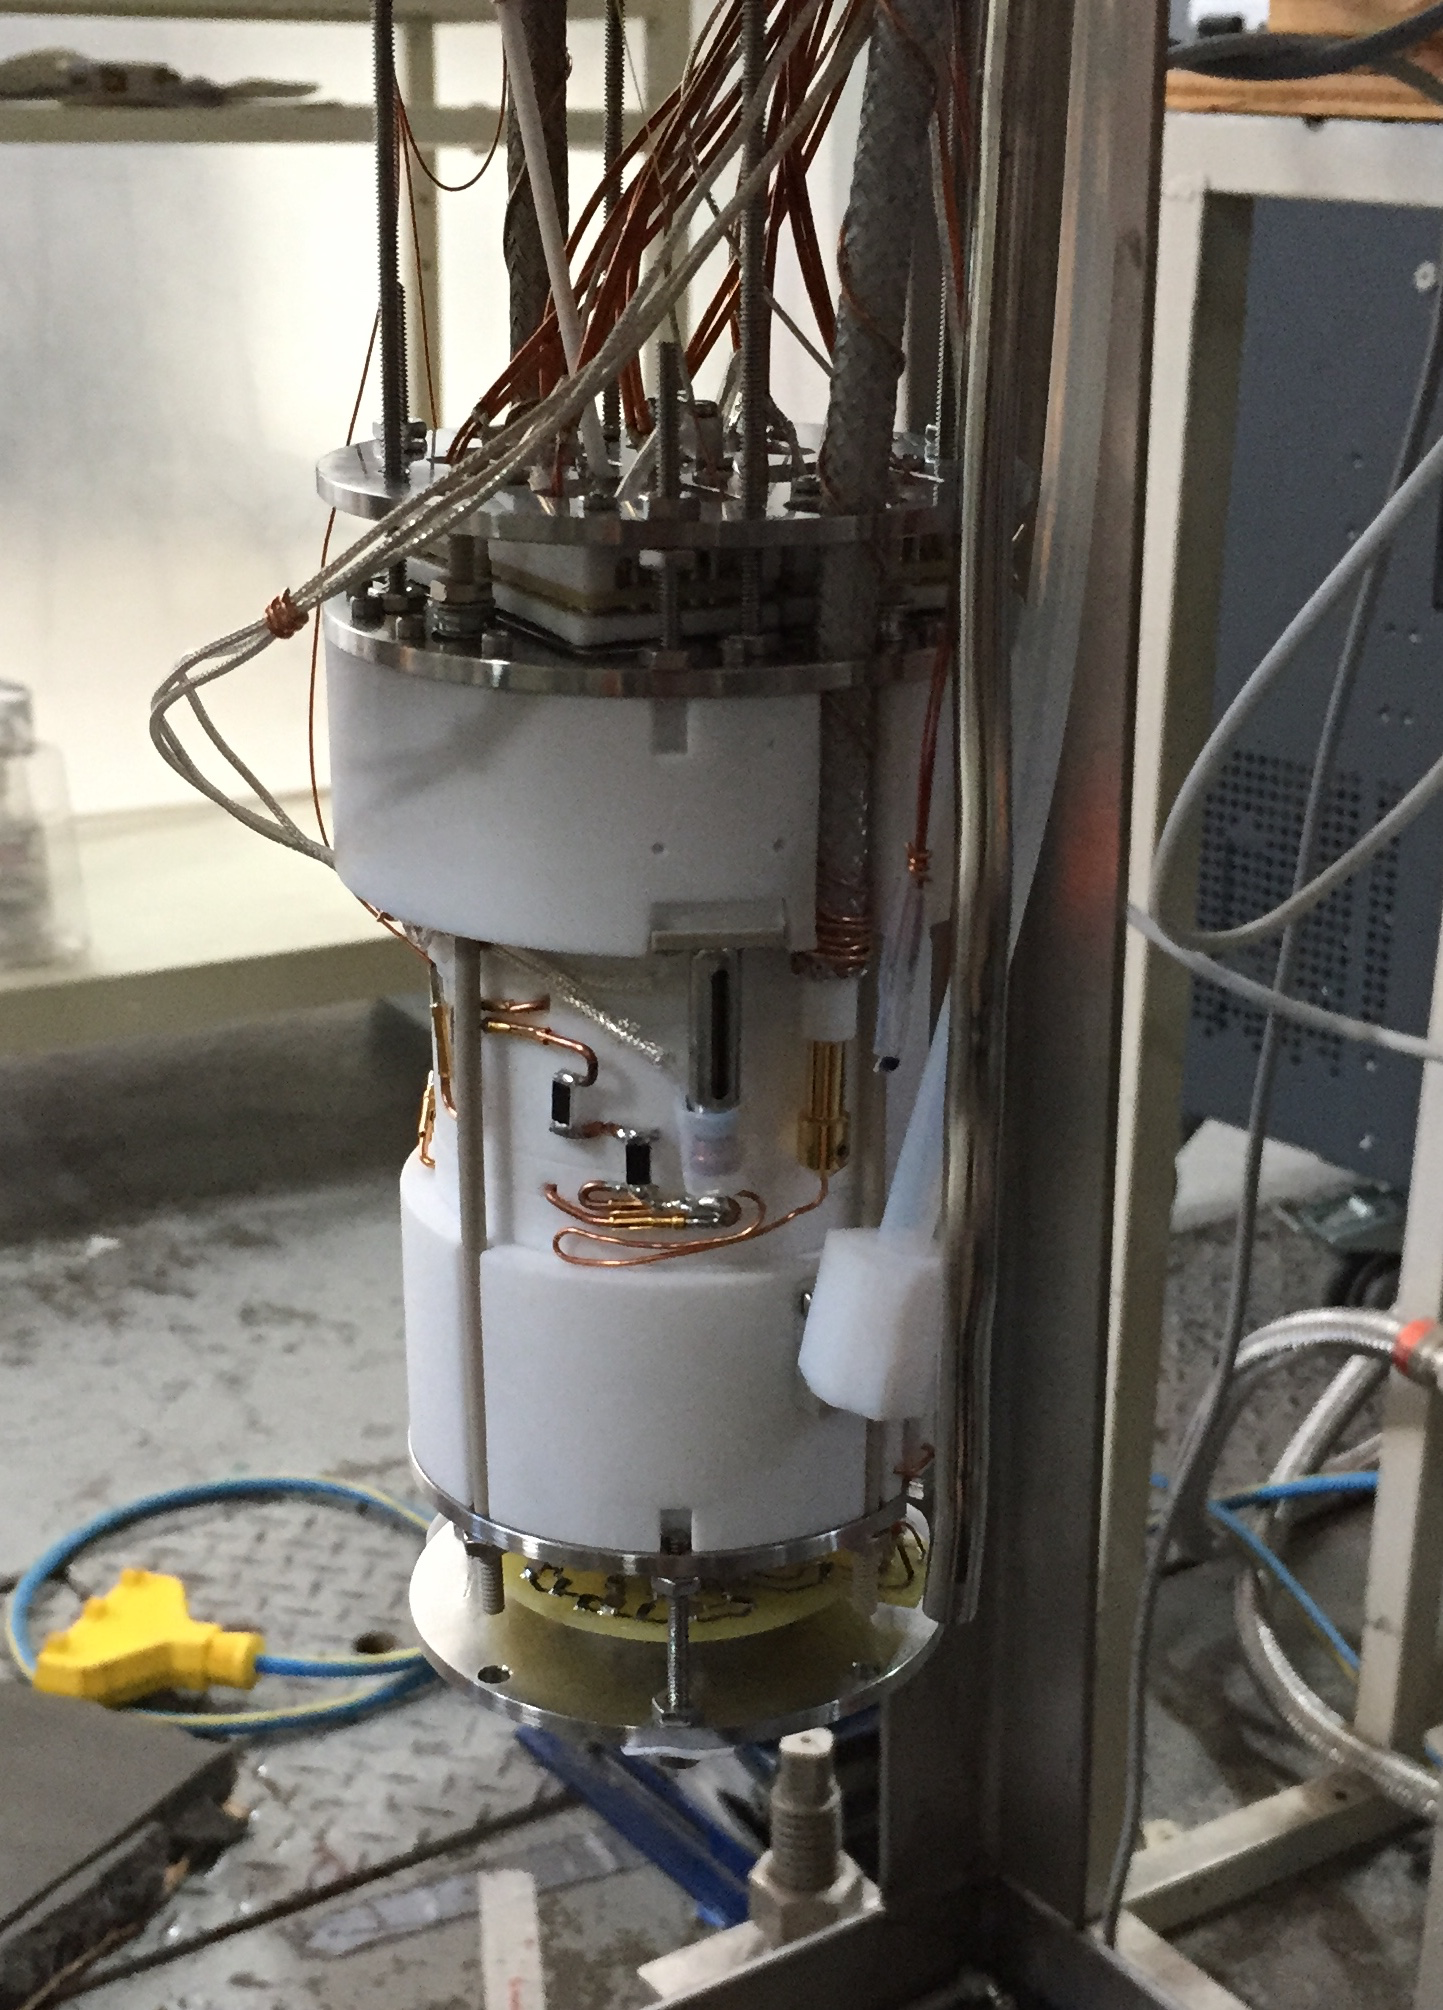
\includegraphics[width=0.48\textwidth]{nerix_tpc_cathode}
	\caption{Two photos of the neriX TPC following routine detector maintenance.  In both photos, one can see the plates holding the single 2'' PMTs (bottom) and the array of four 1'' PMTs (top).  In the left image, one can see the high voltage feedthrough for the anode.  In the right image, one can see the high voltage feedthrough for the cathode and the voltage divider for the field shaping ring.  One can also see the stainless steel pipe used to extract xenon from the inner cryostat's buffer and the plastic tube used to feed re-condensed xenon into the system.}
	\label{fig:nerix_tpc}
\end{figure}



\begin{figure}[t]
        \centering
	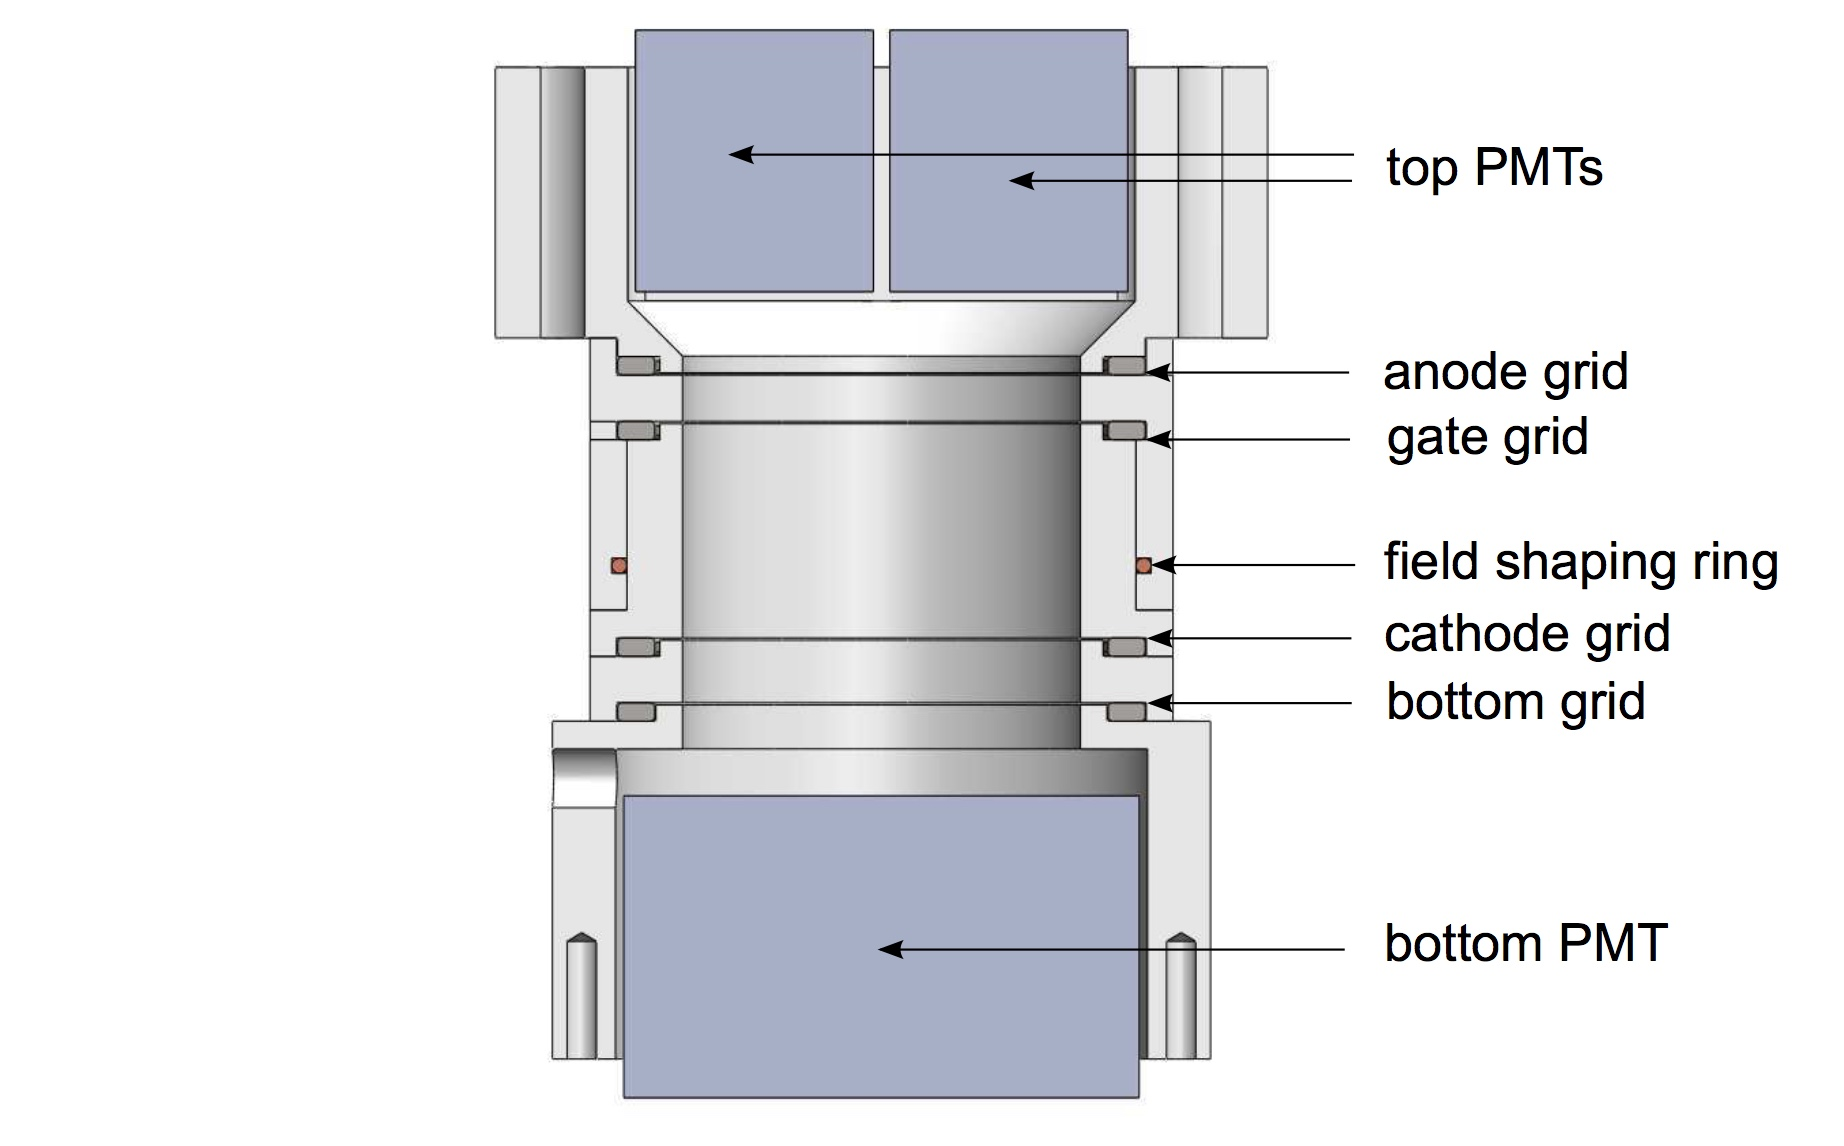
\includegraphics[width=0.8\textwidth]{nerix_tpc_labeled}
	\caption{The neriX TPC with meshes and PMTs labelled.}
	\label{fig:nerix_tpc_labeled}
\end{figure}
   
   
\begin{figure}[bt]
        \centering
	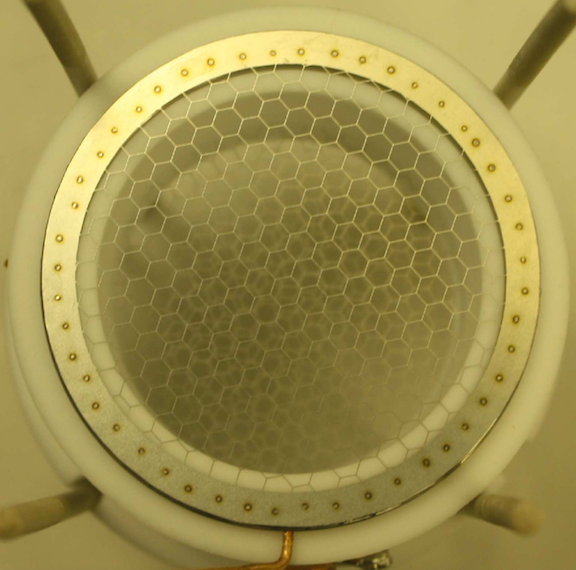
\includegraphics[width=0.5\textwidth]{nerix_tpc_mesh}
	\caption{A photo of one of the meshes used in neriX.}
	\label{fig:nerix_tpc_mesh}
\end{figure}



Six PMTs are installed in neriX: a single 2'' Hamamatsu R6041 PMT is installed below the screening mesh, four 1'' multianode Hamamatsu R8520-M4 PMTs (each with 4 anodes) are installed above the anode mesh, and a single 1'' Hamamatsu R8520-406 is installed in a light-tight stainless steel enclosure located above the TPC.  This final PMT is coupled to the TPC via a 1 mm fiber optic cable placed in between the four 1'' PMTs and is intended for measuring the decay times of singlet and triplet states in liquid xenon (although this measurement was not performed during the nuclear recoil calibration).  Since almost all light from the scintillation signal in the LXe is reflected at the liquid-gas interface, the bottom PMT is the only PMT used for measuring S1 signals.  For simplicity, we also only use the bottom PMT to measure the S2 signals as well (the bottom PMT sees $\sim 50\%$ of the S2 light).  The top PMTs are only used for the position reconstruction of an interaction.

The TPC was connected to the cryostat via a stainless steel motion feedthrough that could be used to raise and lower the detector with a precision of $\sim 25 \, \mu$m.  This motion feedthrough could be used to raise and lower the liquid level relative to the TPC since the liquid level was kept constant via the buffer volume discussed in \secref{sec:nerix_cryostat}.

%The neriX TPC in many ways is very similar to the XENON1T TPC.  Both are made of PTFE (teflon), have meshes to produce


\subsubsection{Cryostat}
\label{sec:nerix_cryostat}

The TPC is surrounded by a double-walled vacuum insulated cryostat.  The inner cryostat was custom made for neriX such that the amount of inactive xenon is minimized.  This inner cryostat, shown in \figref{fig:nerix_cryostat_tpc}, left only approximately 1 cm of space between itself and the TPC with the exception of a $\sim 165 \, \, \textrm{cm}^3$ buffer volume used to maintain the liquid level and the space left for the high voltage feedthroughs.   The inner and outer cryostats are only 1.5 mm thick.  To reduce radiative heat transfer, the inner cryostat is blanketed with mylar in the same way as XENON1T.


\begin{figure}[t]
        \centering
	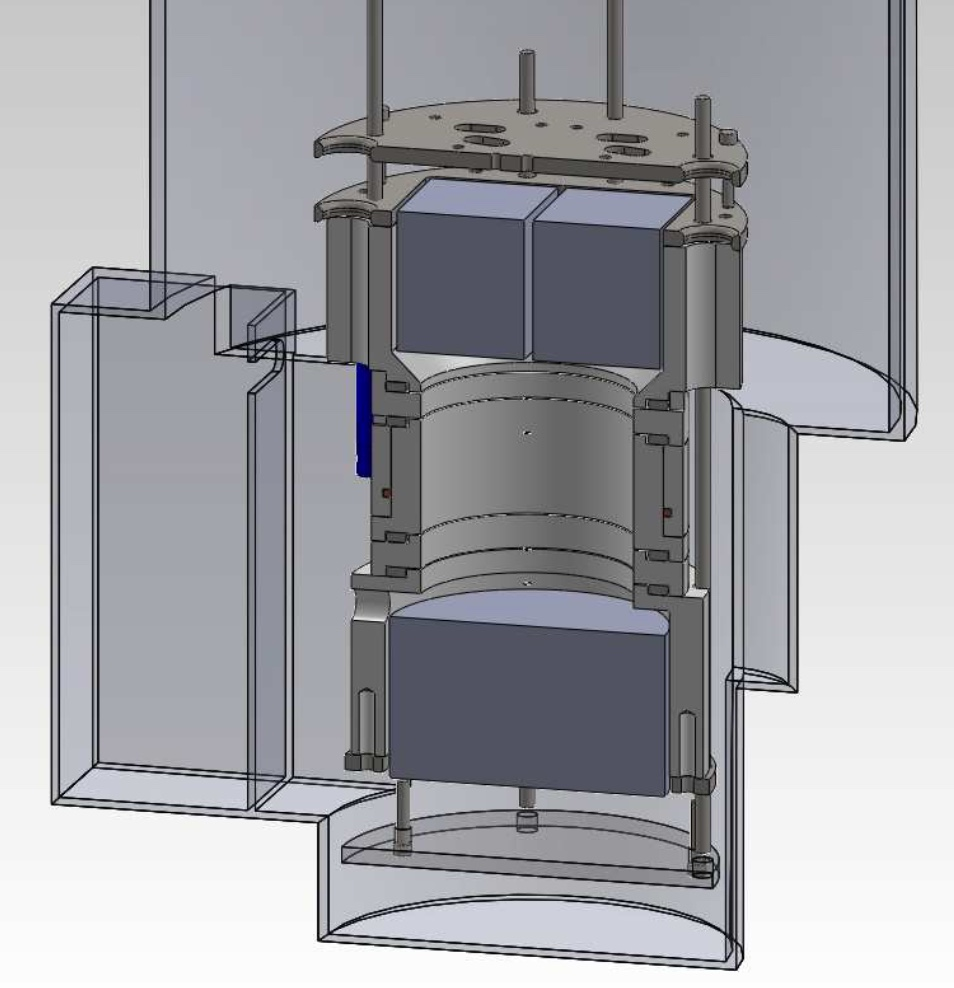
\includegraphics[width=0.5\textwidth]{nerix_cryostat_tpc}
	\caption{The neriX TPC inside of the cryostat.  Note that excluding the buffer volume (left side of the image) and the space left for the high voltage feedthroughs (right side of the image), very little space is left between the cryostat and the TPC, effectively reducing the amount of inactive xenon for undetectable energy losses.}
	\label{fig:nerix_cryostat_tpc}
\end{figure}


\subsubsection{Purification and Cryogenics System}
\label{sec:nerix_cryo_pur}

A diagram of the cryogenics and purification system is shown in \figref{fig:nerix_cryo_pur}.  The cryogenics and purification system used for this measurement is the same as the one used in the measurements of both \citeref{plante2011new} and \citeref{goetzke2016measurement}.

As discussed in earlier chapters, electronegative impurities outgassed from the detector materials will absorb electrons extracted from the interaction site.  Therefore, these impurities must constantly be removed from the xenon to ensure optimal detector operation.  To remove impurities in neriX, the SAES PS4-MT3-R-1 hot getter is used.  Gaseous xenon is flowed through the purification system at approximately 2 SLPM (standard liters per minute) using a KNF N 143 double-diaphragm pump.  A heat exchanger, as described in \citeref{giboni2011xenon}, is used to simultaneously heat up the gaseous xenon coming from the detector and cool down the xenon going towards the detector (from the getter).  This heat exchanger substantially lowers the cooling power required to operate the detector.

To maintain the temperature of the detector, Iwatani PDC08 cold head and SA101 Helium compressor coupled to a copper cold finger are used.  The xenon pressure inside of the cryostat is maintained via resistive heaters thermally connected to the copper cold fingers.  These resistive heaters are controlled by a proportional-integral-derivative (PID) controller that adjusts the power of the heaters to maintain a desired cold-finger temperature.


\begin{figure}[t]
        \centering
	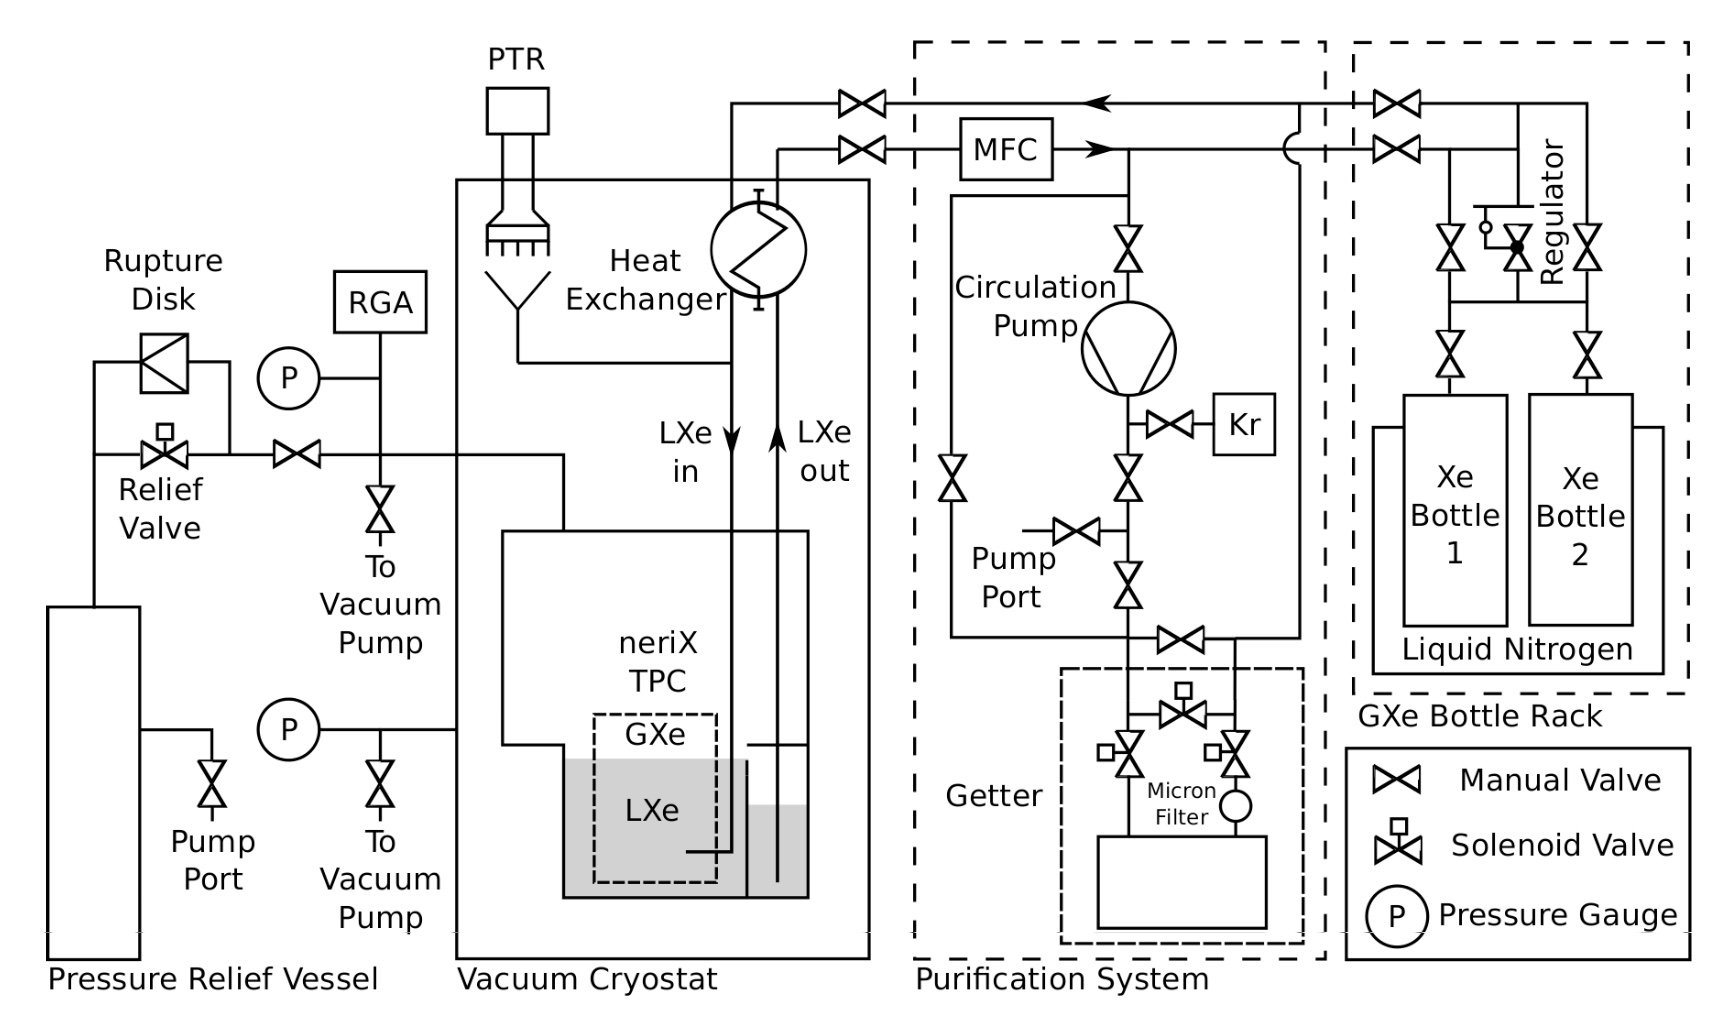
\includegraphics[width=0.99\textwidth]{nerix_cryo_pur}
	\caption{A schematic of the cryogenics and purification system for neriX.  Also shown are the pressure relief system and the xenon storage system.}
	\label{fig:nerix_cryo_pur}
\end{figure}



\subsubsection{Pressure Relief System}
\label{sec:nerix_pressure_relief}

Unlike XENON1T, there is no redundant liquid nitrogen cooling in the event of a power loss for neriX.  This means that if there is a power failure at the laboratory that cooling will be lost and the pressure of the detector will climb.  To prevent damage to the system, especially the PMTs, a pressure relief system was built for neriX.  This pressure relief system consists of a 190 liter stainless steel pressure vessel that is connected to the inner cryostat via a solenoid valve that will open in a controlled manner above a certain pressure in parallel with a rupture disk.  The tank size was chosen such that all of the approximately 2.2 kg of xenon could be stored at room temperature at a pressure below 2.5 bar.  The pressure relief vessel was evacuated on a weekly basis to maintain the chemical purity of the xenon in the case of an emergency.


\subsubsection{Xenon Storage}

The xenon for neriX was stored in two cylinders kept inside of a stainless steel dewar.  When filling the detector, a regulator and a needle valve are used in conjunction with a mass flow meter to keep the detector pressure at reasonable levels.  During recuperation, the dewars are filled with liquid nitrogen such that the xenon inside the bottle freezes and the vapor pressure is low enough to create a cryogenic pump from the cryostat to the storage bottles.  While recuperation can be performed more quickly in an emergency situation, both operations could safely be performed in a single day\footnote{Emptying the detector too quickly could lead to the formation of xenon ice which could damage the bottom PMT so care was always taken to maintain a consistent pressure throughout recuperation in non-emergency situations.}.


\subsubsection{Electric Field Strength and Uniformity}

% ensuring <20\% variation in field to define the fiducial volume

Since the goal of neriX is to measure the light and charge yield of nuclear recoils at different electric fields, it is obviously very important to know what electric field you are measuring the yields for and how uniform it is in the detector.  Unlike in XENON1T, the fiducial volume of neriX is not meant to eliminate background but to exclude regions where the field differs drastically from the mean and where charge can be lost to the wall.  To set the fiducial volume and determine the field strength in neriX, the COMSOL Multiphysics\textsuperscript{\textregistered} Suite was used.  

Simulation details can be found in \citeref{goetzke2015low} but we will present the results of the simulation here.  \tabref{tab:nerix_electric_fields} shows the cathode voltages used along with the corresponding fields given an anode voltage of 4.5 kV, a liquid level 2.5 mm above the gate mesh\footnote{The simulations find that the liquid level has a negligible effect though.}, and the bottom mesh and gate mesh kept at ground.  Simulations found that the variation of the drift field could be kept to within 20\% with a radial cut at approximately 20 cm and cuts in depth at 1 mm below the gate mesh and 0.5 mm above the cathode.  For the nuclear recoil calibration, a more conservative radial cut at 18.25 cm was made.  

\begin{table}[t]
\centering
\def\arraystretch{1.3}
\begin{tabular}{c|ccc}
$\textrm{V}_{\textrm{C}}$ [kV] & -0.345 & -1.054 & -2.356 \\
\hline
$\textrm{E}_{\textrm{D}}$ [kV/cm] & 0.19 & 0.48 & 1.02 \\ 
$\pm 1\sigma$ [kV/cm] & 0.03 & 0.05 & 0.12 \\ 
\end{tabular}
\caption{The different cathode voltages used during the nuclear recoil measurement of neriX and the corresponding electric field strength and field variance.  The simulation assumes an anode voltage of 4.5 kV, a liquid level 2.5 mm above the gate mesh, and the bottom mesh and gate mesh kept at ground.}
\label{tab:nerix_electric_fields}
\end{table}



\subsubsection{Data Acquisition System and Processing}

Raw PMT signals are amplified and then digitized by three CAEN V1724, 14 bit, 100 MS/s flash ADCs (fADC).  Each fADC has a voltage range of 2.25 V, and an input bandwidth of 40 MHz.   Three flash ADCs were required to digitize the 18 PMT signals as well as the multiplexed liquid scintillator signals (multiplexing is discussed in \secref{sec:nerix_daq_trigger}).  The trigger for the data acquisition system used in this measurement will be discussed in \secref{sec:nerix_daq_trigger}.

The data processing system, xerawdp, was originally developed for XENON100 \cite{guillaume_thesis} and modified for neriX.  The processing software was used to reduce the raw waveforms into information about the S1, S2, and liquid scintillator signal sizes and timing.  




\subsection{Neutron Generator}

As mentioned in \secref{sec:nerix_expt_setup}, a small \ce{^2H}$(d, n)$\ce{^3He} generator, shown with a ruler for scale in \figref{fig:nerix_minitron_ruler},  is used to produce neutrons.  This generator is provided by the Schlumberger Princeton Technology Center and will be referred to in this work as the minitron.  The tube of the generator is vacuum sealed and deuterium is produced inside by heating up a replenisher filament.  These deuterium atoms are then ionized via electrons produced from a cathode wire that are accelerated by a grid kept at $\sim 200$ volts.  Deuterium ions are then accelerated towards a titanium-deuteride (\ce{TiD_2}) target where they will either collide with a deuterium atom or be completely stopped.  Deuterium ions that are completely stopped actually replenish the target and thus the target is considered self-regenerating\footnote{The thickness of the target is such that all deuterium ions are stopped.}.  A Heinzinger PNC 100000-3 power supply is used to supply up -100 kV of voltage to accelerate the deuterium ions and to read out the deuterium ion beam current.  A schematic of the minitron electronics is shown in \figref{fig:nerix_minitron_schematic}.

Because the minitron neutron generator utilizes very high voltage, a protective casing was used to prevent disharges from the high voltage connection. The casing was a stainless steel tube with a diameter of approximately 3 inches with teflon, due to its very large dielectric constant, supporting the minitron and filling in almost all excess space in the stainless steel tube.  The small amount of remaining space was filled with mineral oil, which has a higher dielectric constant than air.

The neutron generator used in this work is the same as used in \citeref{plante2011new}.  For more details on the minitron, please refer to \citeref{guillaume_thesis}.


\begin{figure}[t]
        \centering
	\includegraphics[width=0.99\textwidth]{nerix_minitron_ruler}
	\caption{The deuterium-deuterium neutron generator used to produce 2.45 MeV neutrons.}
	\label{fig:nerix_minitron_ruler}
\end{figure}


\begin{figure}[bt]
        \centering
	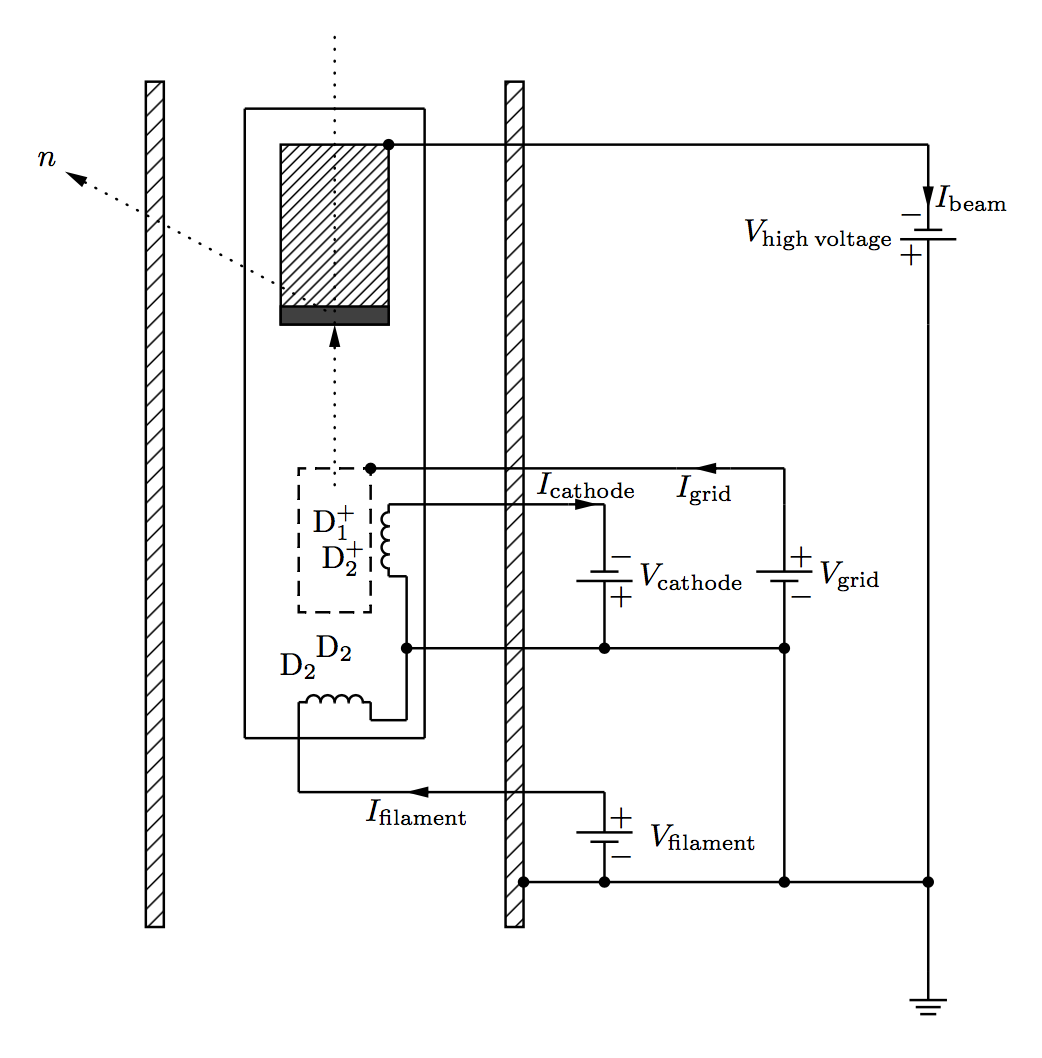
\includegraphics[width=0.65\textwidth]{nerix_minitron_schematic}
	\caption{The electronics of the minitron neutron generator.  Image Credit: \citeref{guillaume_thesis}.}
	\label{fig:nerix_minitron_schematic}
\end{figure}


\begin{figure}[t]
	\centering
	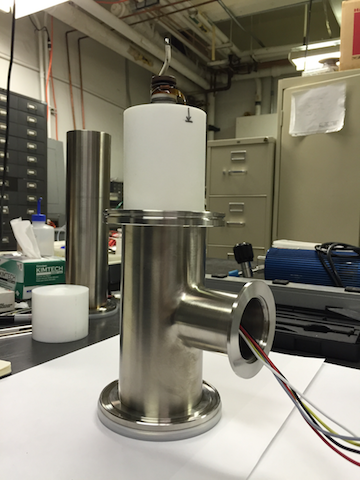
\includegraphics[width=0.533\textwidth]{nerix_minitron_partial_case}
	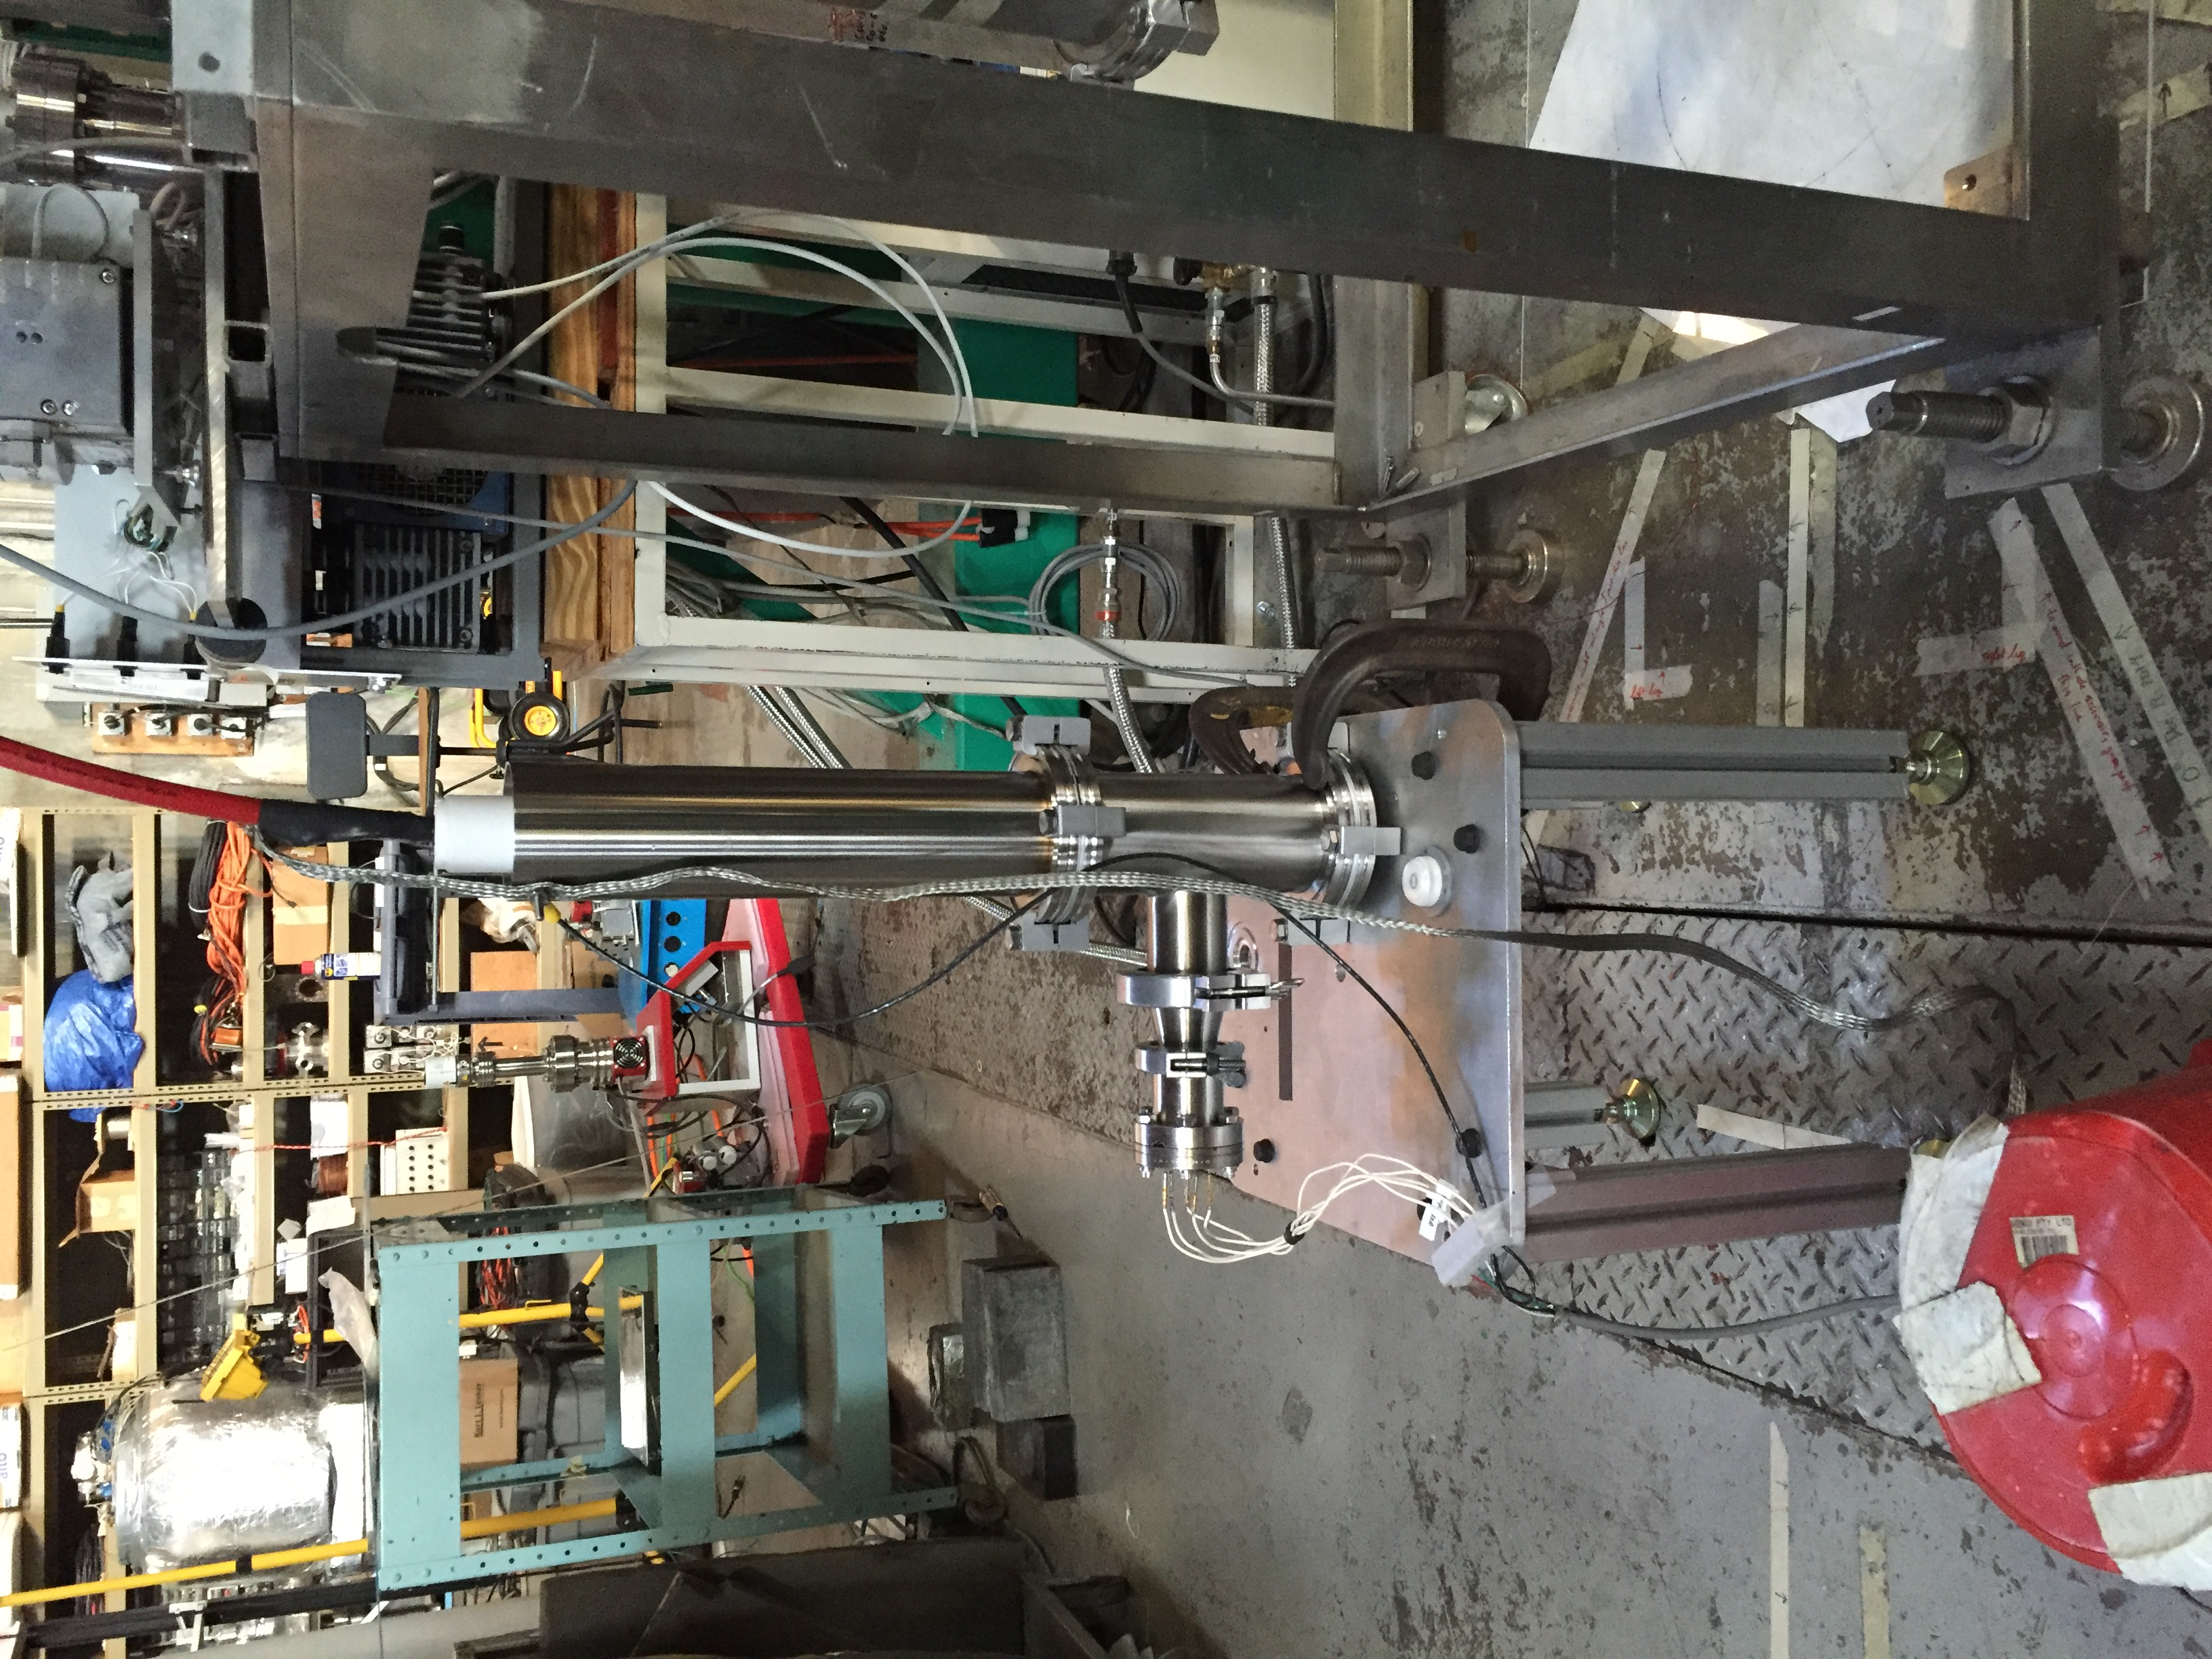
\includegraphics[width=0.4\textwidth]{nerix_minitron_set}
	\caption{On the left, the minitron in its partially constructed case.  Notice that the teflon leaves very little room between the steel and minitron to maximize the potential voltage that can be used without causing an electrical breakdown.  On the right, the minitron in its final set position.  While not visible, the minitron case has been filled with mineral oil at this point to reduce risk of electrical breakdowns.}
	\label{fig:nerix_minitron_rate}
\end{figure}


\subsubsection{Neutron Energy Spectrum}

For non-relativistic deuterons,  the energy of the neutron produced from a deuterium-deuterium interaction is only dependent on the scattering angle and the energy of the deuteron.  The exact energy, in this case, is given by \eqnref{eqn:nerix_neutron_energy} \cite{csikai1987crc}. 

\begin{equation}
        \label{eqn:nerix_neutron_energy}
        \begin{split}
                E_n^{\sfrac{1}{2}} = \frac{(m_d m_n E_d)^{\sfrac{1}{2}}}{m_{\textrm{He}} + m_n} \textrm{cos} \, \varphi  + \frac{\left[ m_d m_n E_d \, \textrm{cos}^2 \, \varphi + (m_{\textrm{He}} + m_n) [ m_{\textrm{He}} Q + (m_{\textrm{He}} - m_d) E_d ] \right]^{\sfrac{1}{2}}}{m_{\textrm{He}} + m_n}
        \end{split}
\end{equation}

In \eqnref{eqn:nerix_neutron_energy}, $m_{\textrm{He}}$, $m_n$, and $m_d$ are the masses of helium, neutrons, and deuterium, respectively, $Q$ is the $Q$-value of the reaction (3.269 MeV), and $\varphi$ is the emission angle of the neutron in the laboratory frame.  To approximate the energy spectrum as a function of the scattering angle and deuteron energy, we say that the yield as a function of these variables is proportional to the differential cross-section multiplied by the distribution of incident deuteron energies, $f(E_d)$\footnote{This derivation of the angular dependence of the neutron energy spectrum is from Qing Lin (current institution: Columbia University)}.  We could assume that this distribution of deuteron energies is a delta function for the fixed target collision but this would ignore all of the other interactions that can occur in the \titde{}.  

\begin{equation}
        \frac{d^2 N}{d E_d d \varphi} \sim \frac{d \sigma}{d \varphi} f(E_d)
\end{equation}

Since the energy of the deuteron is directly related to the energy of the neutron produced by \eqnref{eqn:nerix_neutron_energy}, we can rewrite the above equation in terms of the neutron energy and the emission angle.

\begin{equation}
        \frac{d^2 N}{d E_n d \varphi} \sim \frac{d \sigma}{d \varphi} f(E_d) \left( \frac{\partial E_n}{\partial E_d} \right)^{-1}
\end{equation}

We now define two variables: $\sigma_n$, the total cross-section of deuterium-deuterium fusion into a neutron, and $\sigma_{\textrm{tot}}$, the total cross-section of all possible interactions.  It turns out that $\sigma_{\textrm{tot}} \gg \sigma_n$ due to Rutherford scattering.  Therefore, we say that probability of a neutron being produced per interaction is given by $p = \frac{\sigma_n}{\sigma_{\textrm{tot}}}$.  We say that the number of interactions is approximately given by the energy lost, $E_l$, divided by the average interaction energy, $W$.  We define $W$ in terms of the stopping power such that $W = \frac{dE / dx(E_d) \cdot M}{\sigma_{\textrm{tot}} N_a}$, where $N_a$ is Avogadro's number and $M$ is the molar mass of \titde{}.

Therefore, we approximate the probability that the incoming deuteron fuses with a deuteron in the target after $i = \frac{E_l}{W}$ interactions is given by \eqnref{eqn:nerix_minitron_energy_loss_1}.

\begin{equation}
        \label{eqn:nerix_minitron_energy_loss_1}
        f(E_l) \sim \left( 1 - \frac{\sigma_n}{\sigma_{\textrm{tot}}} \right)^i = \left( 1 - \frac{\sigma_n}{\sigma_{\textrm{tot}}} \right)^{E_l \cdot \frac{\sigma_{\textrm{tot}} N_a}{dE / dx(E_d) \cdot M}}
\end{equation}

This expression for the distribution of the energy lost by the incoming deuteron can be rearranged into a more convenient form.

\begin{equation}
        \label{eqn:nerix_minitron_energy_loss_2}
         f(E_l) \sim \left[ \left( 1 - \frac{1}{\frac{\sigma_{\textrm{tot}}}{\sigma_n}} \right)^{\frac{\sigma_{\textrm{tot}}}{\sigma_n}} \right] ^{E_l \cdot \frac{\sigma_n N_a}{dE / dx(E_d) \cdot M}} \approx e^{-E_l \cdot \frac{\sigma_n N_a}{dE / dx(E_d) \cdot M}}
\end{equation}

With an approximate distribution for the energy loss, and therefore the deuteron energy during the fusion interaction, we can simulate our expected angular distribution \cite{chadwick2011endf, guillaume_thesis}.  The angular distribution assuming an incoming deuteron energy of 80 keV is shown in \figref{fig:nerix_yield_emission_angle}.

\begin{figure}[t]
        \centering
	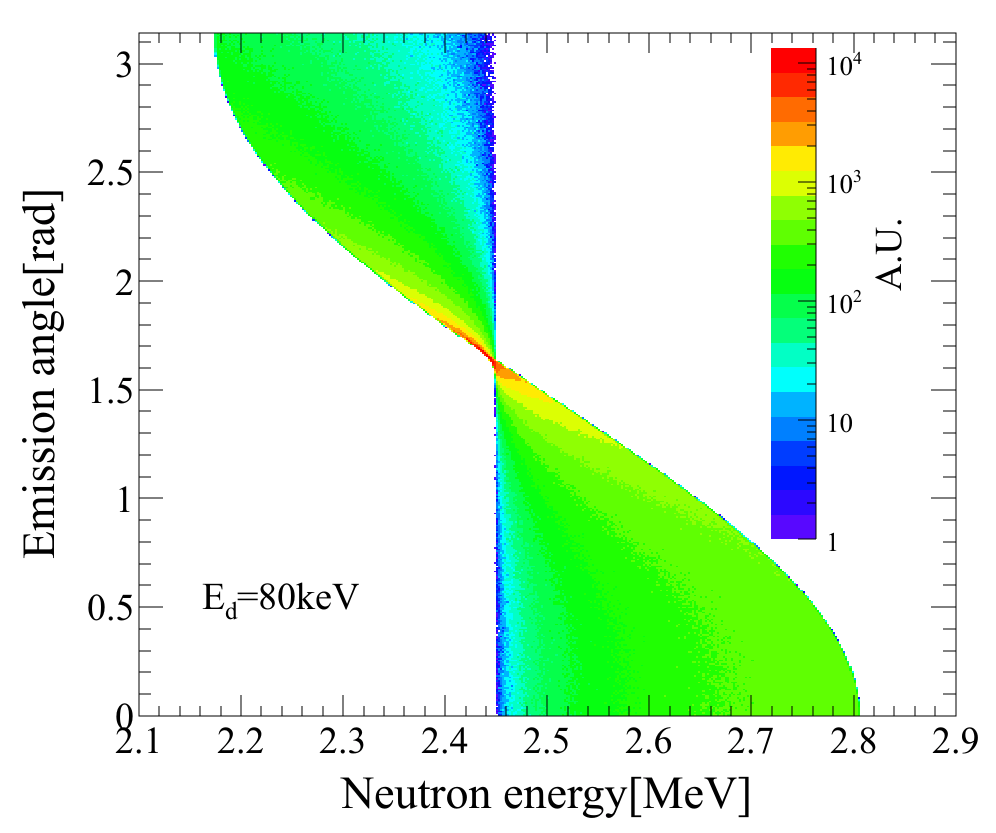
\includegraphics[width=0.75\textwidth]{nerix_yield_emission_angle}
	\caption{The expected angular distribution of neutrons as a function of emission angle for a maximum deuteron energy of 80 keV.}
	\label{fig:nerix_yield_emission_angle}
\end{figure}





\subsubsection{Neutron Yield}

While ultimately we did not include the neutron rate in our analysis of the yields, we did characterize the neutron generator to ensure that it was operating as expected.  \citeref{guillaume_thesis}, following the analysis from \citeref{csikai1987crc}, shows that the flux of neutrons generated should increase approximately exponentially with the high voltage used to accelerate the ionized deuterium atoms and molecules and linearly with the deuterium ion beam current.  We assume that these two effects are uncorrelated and therefore the neutron production rate can be written as $\frac{dN}{dt} = f(I)g(V)$ where $f(I)$ describes the rate's dependence on the beam current and $g(V)$ describes the rate's dependence on the high voltage.

The neutron flux of the minitron neutron generator was measured using a Nuclear Research Corporation NP-2 portable neutron monitor \cite{np2_manual}.  The NP-2 neutron monitor uses a \ce{BF_3} target housed inside of a polyethylene moderator that attenuates the fast neutrons such that they can be counted.  The detector measures in units of dose rate which can be converted to flux by means of the fluence per unit dose equivalent of 2.45 MeV neutrons.  As mentioned, we approximated that the current and high voltage could be treated separately and measured the change in one while holding the other fixed to characterize the neutron flux.  For the measurement, the NP-2 detector was placed 180 cm away from the neutron generator (inside of its case) and at an angle of $\frac{\pi}{2}$ relative to the minitron.  The rate measurements were then used to fit rate as a function of beam current and voltage (shown in \figref{fig:nerix_minitron_fits}).  Using these functions, we can then predict the neutron flux of the minitron, as shown in \figref{fig:nerix_minitron_rate}.

%shielding oil teflon etc

\begin{figure}[p]
	\centering
	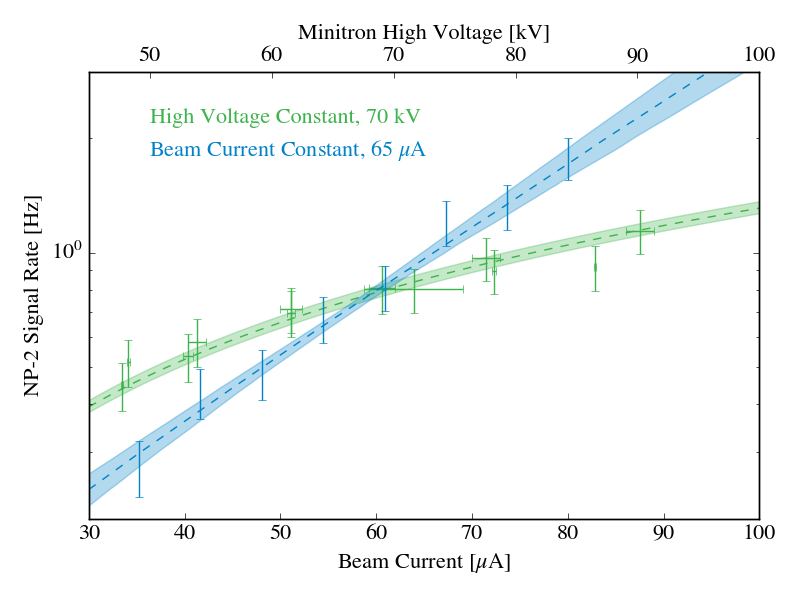
\includegraphics[width=0.8\textwidth]{nerix_minitron_fits}
	\caption{The NP-2 neutron detector signal rate as a function of beam current, holding the high voltage fixed, and high voltage, holding the beam current fixed.  Shaded regions represents 68\% credible region while dotted lines show the best fits.}
	\label{fig:nerix_minitron_fits}

        \vspace{\floatsep}

	\centering
	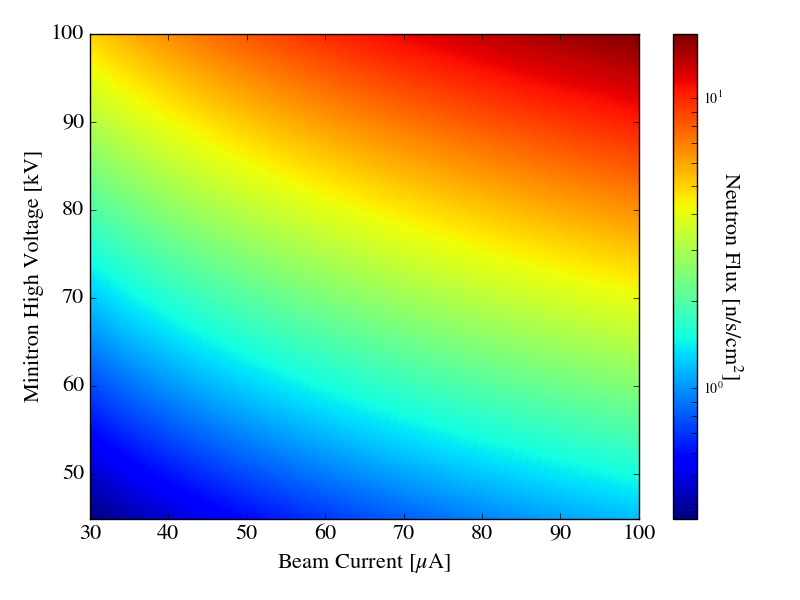
\includegraphics[width=0.8\textwidth]{nerix_minitron_rate}
	\caption{The expected neutron flux from the minitron neutron generator at a distance of 180 cm at an angle of $\frac{\pi}{2}$.}
	\label{fig:nerix_minitron_rate}
\end{figure}



\subsection{Liquid Scintillators}

In theory, any detector of ionizing radiation could act as the secondary detector in a nuclear recoil calibration.  In practice, however, the gamma ray background rate is large enough in a laboratory setting that detectors with high levels of discrimination are needed to differentiate neutrons from background in the secondary detector.  

For this measurement, the M510 detectors from Eljen Technologies were used.  The M510 detector is filled with the liquid scintillator EJ301, chosen for its excellent pulse shape discrimination properties.  The EJ301 compound has three characteristic decay times: 3.16, 32.3, and 270 ns \cite{kuchnir1968time, ej301_manual}.  The first two states are related to the excitation of electrons to the singlet and triplet state, respectively, while the slowest decay time is from the delayed fluorescence of the triplet state \cite{lang2017improved}.  Nuclear recoils in the liquid scintillator will exhibit much longer decay times than electronic recoils caused by gamma rays.  

An initial characterization of the liquid scintillators was performed to determine the optimal voltage and integration window for nuclear and electronic recoil discrimination and calibrations were performed several times over the course of the run to ensure performance was still adequate.  An example of the pulse discrimination from one the M510 detectors from coincidence data is shown in \figref{fig:nerix_ej_discrimination}.  Similar to \citeref{guillaume_thesis}, we set a threshold in the detectors' pulse size where discrimination is poor - however this was done via the hardware trigger and not a software cut to reduce data intake. 

\begin{figure}[t]
        \centering
	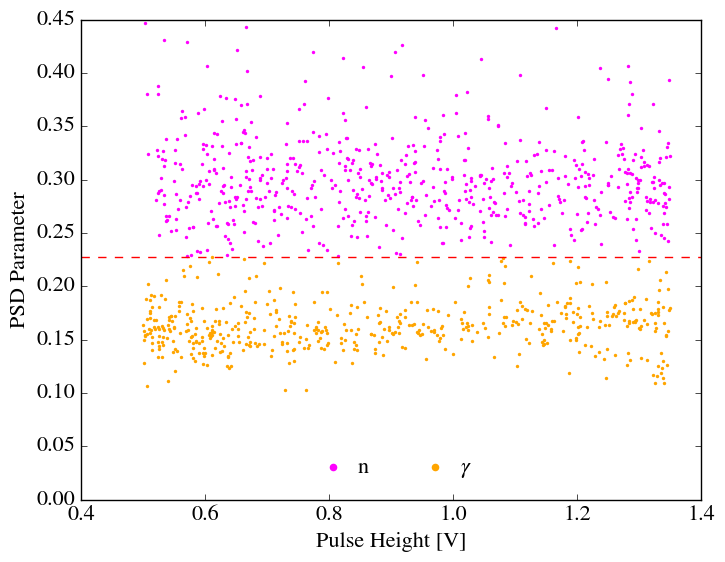
\includegraphics[width=0.75\textwidth]{nerix_coin_ej}
	\caption{Discrimination space for one of the four M510 detectors from coincidence data.  Notice that a hardware cut is made via a threshold discriminator at approximately 500 mV in order to remove events with poor pulse shape discrimination.}
	\label{fig:nerix_ej_discrimination}
\end{figure}

A fifth and smaller version of the M510 detector was placed 180 cm away from the neutron generator to monitor the minitron rate at all times.



\subsection{Data Acquisition System}
\label{sec:nerix_daq_trigger}

A schematic of each of these triggers is shown in \figref{fig:nerix_daq_trigger_setup} and the details of each are given below.

The data acquisition system for this measurement is identical to the one described in \citeref{goetzke2016measurement}.  The system consisted of three 14-bit flash ADCs (model v1724 from CAEN) at 100 MS/s with 40 MHz bandwidth.  When a trigger pulse was received by the VME crate controller, this memory would be written to the disk of our data acquisition server.  The data acquisition server used was synchronized to a storage and processing server where data could be further analyzed.

All of the top signals are fed directly into 10x amplifiers which are then immediately fed into digitizer channels.  The bottom PMT signal is the only channel used to form the trigger since it sees the majority of the light in the detector.  The bottom PMT's signal is fed into a CAEN voltage divider.  One of these two signals is sent directly to the digitizer unamplified (to avoid digitizer saturation in large S2 signals) while the other copy of the signal is sent to a 10x amplifier where two copies are made.  One of these two copies is sent directly to the digitizer while the other is sent to an updating threshold discriminator.  This updating threshold discriminator produces a NIM pulse for as long as the signal is above the set threshold (5.16 mV for this measurement) making the width in time of the NIM pulse approximately the same as the width of the true signal.  The output from the updating threshold discriminator is considered to be our S1 trigger.  

The S1 trigger is used as the main building block for the S2 trigger.  The S1 trigger is sent into a logic fan.  One copy from the logic fan is sent to a variable width gate generator (set at 400 ns for this measurement) while the other is sent into a 24 ns delay.  The gate generator produces a \nimbar{} pulse that is combined in a logical AND with the delayed S1 trigger.  In this way, only S1 triggers wider than the gate will cause a new trigger\footnote{The delay is needed because the gate takes approximately 10 ns to create.}.  If the logical AND results in a pulse this is considered an S2 trigger (S2 pulses in general are much wider than S1 pulses).  The width of the S2 trigger pulse is set to be 29.5 $\mu$s for reasons that will be explained shortly.

This S2 trigger is passed into a logical fan where three copies are made.  One is sent into a gate generator that produces a 100 $\mu$s \nimbar{} pulse.  The \nimbar{} pulse is combined with another copy of the S2 trigger in a logical AND.  Since there is no delay on the S2 pulse, the original S2 trigger will result in an output pulse however S2s occurring after the current S2 and before the end of the \nimbar{} pulse will not produce an output pulse based on the logical AND.  This therefore limits the maximum rate of triggers to one over the gate width (although typical data acquisition rates are $< 100$ Hz).   The output signal from this logical AND is called the S2 hold-off trigger.

Four M510 detectors were used simultaneously such that two energy spectra could be measured at a time.  Since the rate of signals in the liquid scintillators was low relative to the TPC, it was decided to use a single digitizer channel to capture all of the EJ pulses via multiplexing.  The signals from the PMTs in the M510 detectors were first sent to a 10x amplifier where two amplified copies were produced.  The first copy of the M510 signals was sent into a linear fan.  The second copy of each of amplified M510 signals went to a threshold discriminator.  The threshold was decided on a detector-by-detector basis such that signal sizes were eliminated where we had little discrimination power between nuclear and electronic recoils.  Two copies of the output from the threshold discriminator were created.  The first copy of each signal was sent into a delay generator that delays the logic pulse by a time unique to each detector (for example, one of the M510s' triggers was delayed by 6 $\mu$s while another was delayed by 7 $\mu$s).  The delayed triggers are then sent into the same linear fan as the original pulses.  In this way, the processor can determine which M510 detector the signal came from based on where the M510 trigger is found in the waveform.  

As was mentioned, the threshold discriminator for the M510 detectors creates two copies of each trigger.  The second copy of these triggers is sent into a logical OR to produce a single logic signal.  This logic signal is then delayed 28 $\mu$s and combined in a logical AND with the 29 $\mu$s S2 gate.  The output of the logical AND forms our coincidence trigger.  The long delay and gate may seem unnecessary at first but are actually needed since the M510 signal is very close in time to the S1 and not the S2.  This means that the S2 signal can occur tens of $\mu$s after the M510 trigger is created.  Therefore, by creating a gate on the S2 and delaying the M510 trigger we ensure that we will not lose any good events due to the electron drift time in the TPC.  




\begin{figure}[p]
        \centering
	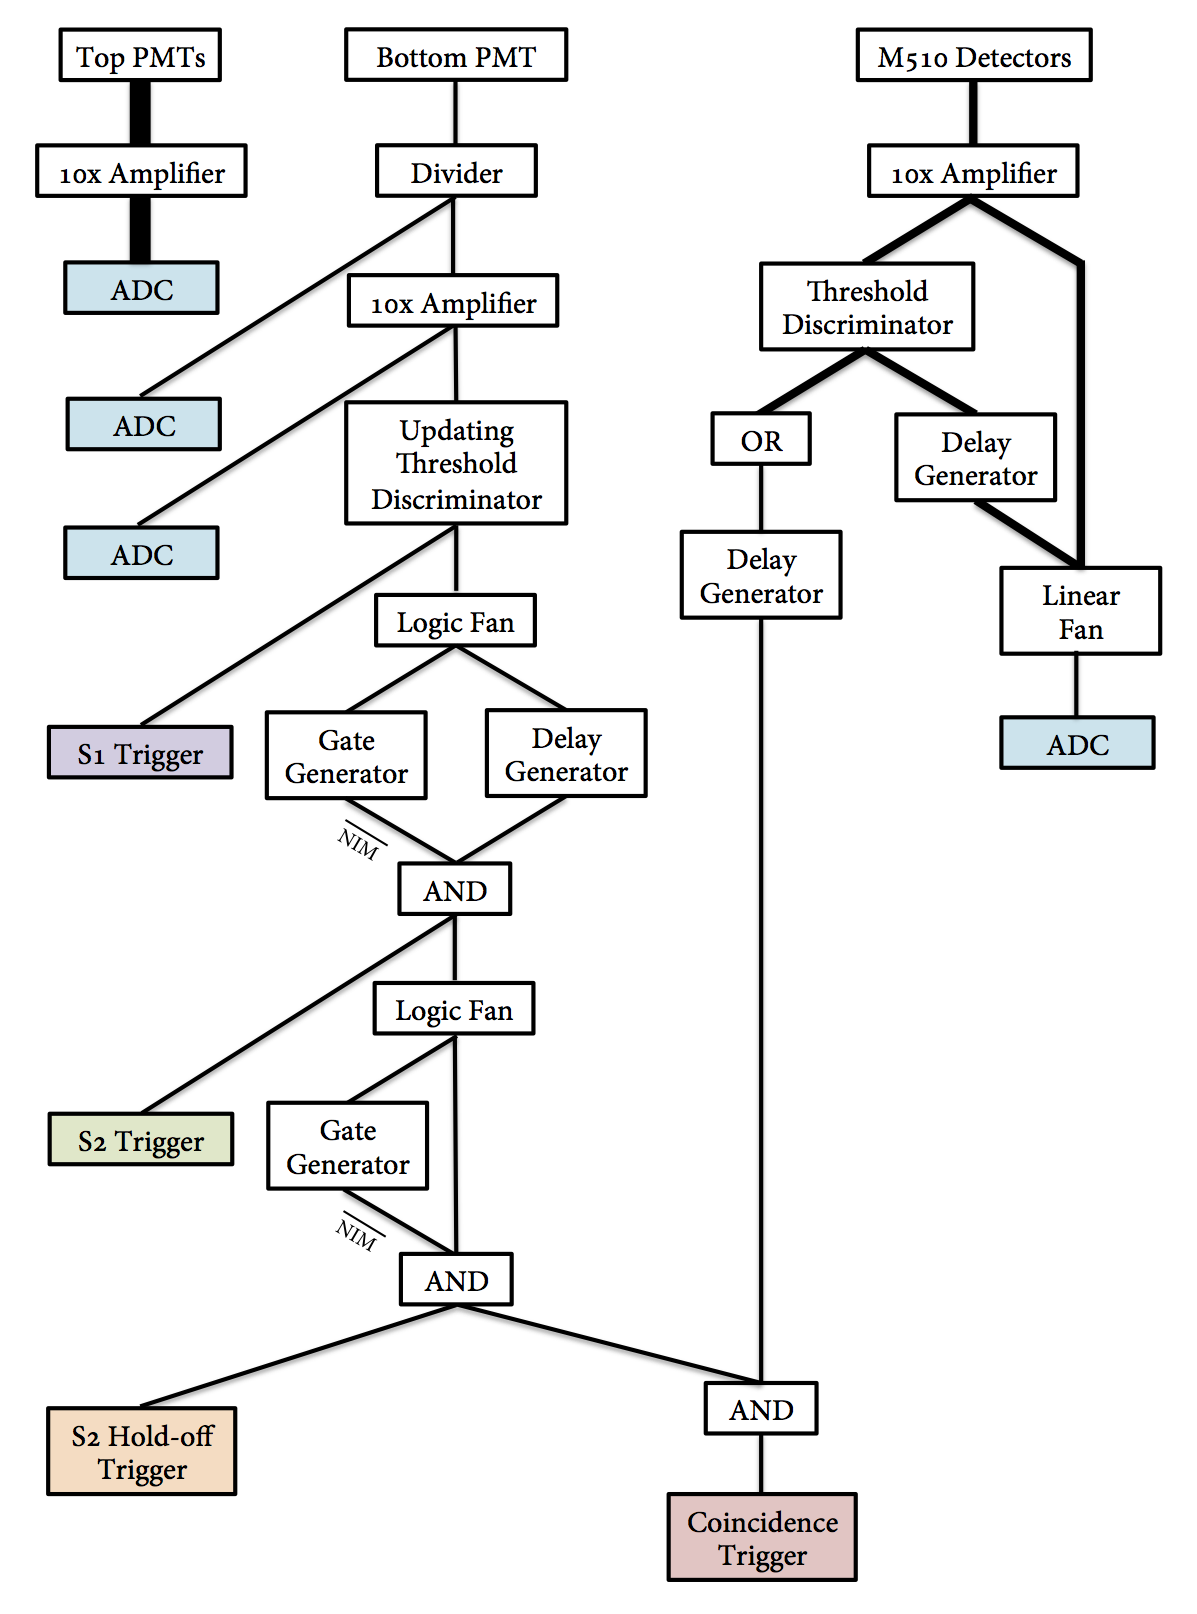
\includegraphics[width=0.99\textwidth]{nerix_daq_trigger_setup}
	\caption{The trigger schematic for the neriX nuclear recoil measurement.  For details on the triggers please refer to the text in \secref{sec:nerix_daq_trigger}.}
	\label{fig:nerix_daq_trigger_setup}
\end{figure}

\section{Characterization and Calibration of neriX}
\label{sec:nerix_cals}

As mentioned in chapters two and three, the process from energy deposition to the S1 and S2 signal read out of a waveform for analysis can essentially be broken down into two subsections: the signal production and the detector physics.  If we want to measure the physics of the signal production mechanism, we must be able to decouple the detector physics.  To do this, we must make independent measurements to characterize the detector as best as we can.  

While many of the properties of the detector we are trying to characterize are the same as XENON1T, there are some differences in how we carry out the measurements simply due to the scale of XENON1T relative to neriX.



\subsection{PMT Characterization}

As in XENON1T, the most basic task in characterizing the TPC is the PMT calibration.  The goal of the PMT calibration is to understand the response of a PMT to incident photons.  This task is typically performed by examining the response of the PMT to a single photoelectron (single electron ejected at the photocathode as the result of an incident photon) since larger signals can be estimated via the convolution of multiple single photoelectron response functions.  Ideally, we would like to completely understand the shape of the response function of the PMT but at the same time, most experiments settle for the mean and variance of the response (since by the central limit theorem these will describe the response for large numbers of photons).  %However, since we wish to understand the low energy response of nuclear recoils, which will involve very small signals ($< 10$ PE), we cannot settle for knowing only the mean and variance.

As in XENON1T, the low light calibration of PMTs is performed using a blue LED pulse generated by a digital pulse generator (BNC PB-5) and fed into the detector via a fiber optic cable.  The standard way of calibrating a PMT in this type of experiment is to use a low light level (such that the given PMT only sees a signal 5--10\% of the time) and either fit the data using a Gaussian model of the response or extract the mean and variance according to the statistical treatment in \citeref{saldanha2017model}.  However, neither of these was satisfactory: the former was not satisfactory as it resulted in an unphysical signal for the PMT response approximately 15\% of the time (since the Gaussian distribution is not bounded below by zero) and therefore has a large potential for bias and the latter was not satisfactory given that we could not guarantee identical operating conditions between the background-only data and pulser data, a required condition for the statistical approach.  Therefore, a new model was developed by the author, called the \textit{cascade model}, which tries to simulate the actual physics of a PMT including the underamplification of electrons and its dynode structure \cite{anthony2017characterization}.  This model is discussed in further detail in \appref{app:pmts} and uses a GPU-based analysis framework, like the measurement of the light and charge yield in neriX (the focus of this chapter) and the electronic and nuclear recoil calibration of XENON1T (discussed in \secref{sec:xe1t_er_nr_calibration}), that will be discussed in \appref{app:gpus}.  Unlike the other two calibration methods, it is actually more effective to use a higher light level such that 1--2 photoelectrons are seen on average\footnote{This does not affect the assumption that the number of photoelectrons seen follows a Poisson distribution that is standard in these types of measurements.}.  A sample low-light spectrum is shown in \figref{fig:nerix_pmt_best_fit} along with the best fits and 68\% credible regions of both the Gaussian and cascade models.  From this spectrum alone, it does not appear that the cascade model is a significant improvement but if one looks at \figref{fig:nerix_spe_response}, which shows the full-amplification SPE spectrum for both models, one can see the reason why the Gaussian model is not acceptable: it results in a negative signal a non-negligible fraction of the time.


\begin{figure}[p]
	\centering
	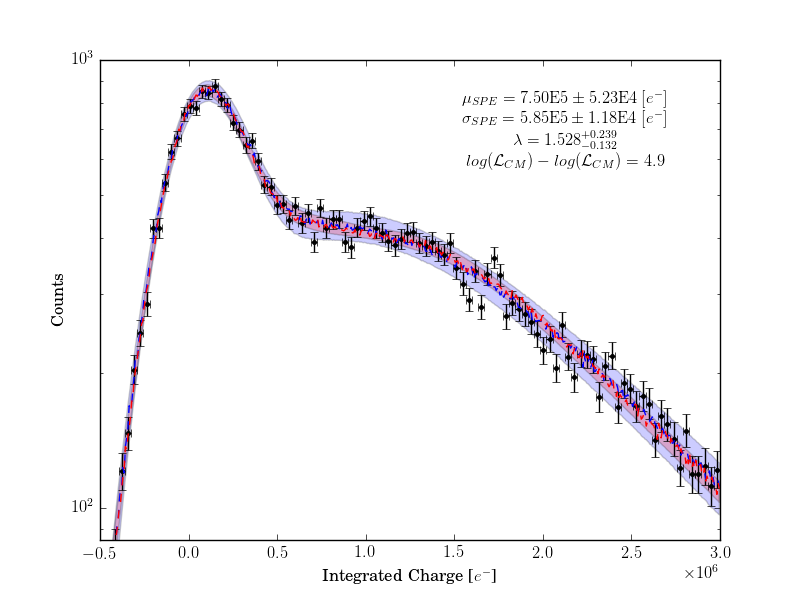
\includegraphics[width=0.7\textwidth]{nerix_pmt_best_fit}
	\caption{The fit of the cascade (blue) and Gaussian (red) single photoelectron response model for the bottom PMT at 800 V.  The statistics shown are for the cascade model which results in a marginally better fit as can be seen from the log likelihood difference.  The dotted lines shown are the best fits and the shaded region is the 68\% credible region.}
	\label{fig:nerix_pmt_best_fit}

        \vspace{\floatsep}

	\centering
	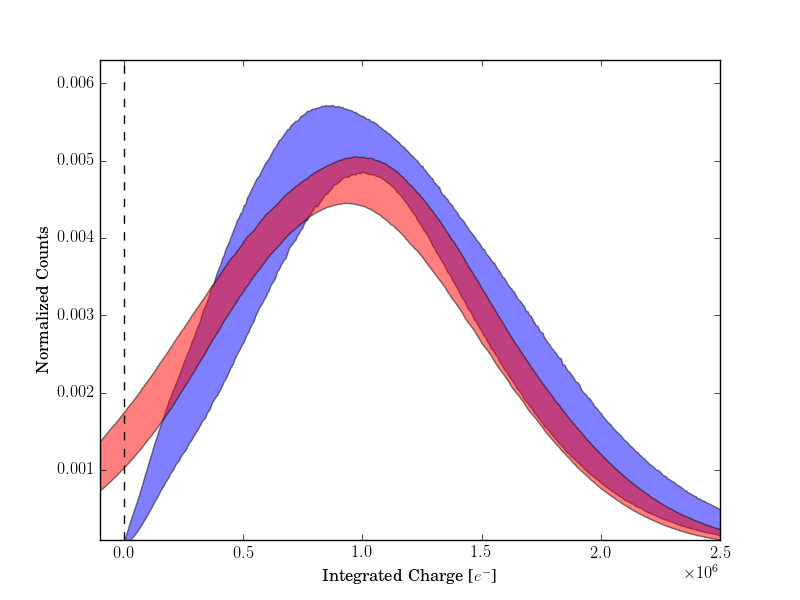
\includegraphics[width=0.7\textwidth]{nerix_spe_response}
	\caption{The 68\% credible region for the single photoelectron response for fully-amplified electrons for the bottom PMT at 800 V.  Notice that the Gaussian model (red) results in a non-physical response a non-negligible fraction of the time while the cascade model (blue) does not exhibit this behavior.}
	\label{fig:nerix_spe_response}
\end{figure}


Unlike \citeref{goetzke2016measurement}, no gain instability was seen during this measurement in neriX.  

To avoid issues of saturation with the PMTs, nuclear recoil data was taken with PMT gains ranging from $5-10 \cdot 10^5 \, \, e^-$ while electronic recoil data where our concern was the full absorption peak (like the anticorrelation analysis in \secref{sec:nerix_anticorrelation}) was taken with gains two orders of magnitude smaller.  Even using our GPU-based cascade model it is extremely difficult to fit such a small PMT response.  Therefore, we used what is referred to in \citeref{goetzke2015low} as the MPE method.  To use the MPE method you must first calibrate the response of the PMT at its normal operating voltage.  Following a standard calibration, you illuminate the same PMT at the same voltage with a high light level and use the gain found from before to estimate the mean number of photoelectrons.  You then reduce the PMT voltage and remeasure the response of the PMT to the high light level.  Since the mean number of photoelectrons observed should be independent of voltage, you can use the response at the lower voltage and high light level to extract the gain of the PMT at a much lower voltage.

When measuring this effect, we varied the bottom PMT voltage from 800 V, our standard operating voltage, down to 500 V.  At approximately 600 V, saturation effects in the 662 keV peak were no longer present.  Ideally, one would expect the gain to decrease exponentially with voltage, however we noticed a significant deviation from this behavior.  We believe that this deviation is due in part to the decreasing collection efficiency of photoelectrons of the PMT at lower voltages, an effect described in \citeref{carter1980photomultiplier}.  While the voltage dependence of the effect is PMT dependent, we multiplied our power law by a generic second-order polynomial efficiency function in an attempt to describe it.  The best fit of both the gain and collection efficiency are shown in \figref{fig:nerix_mpe}.

\begin{figure}[t]
        \centering
	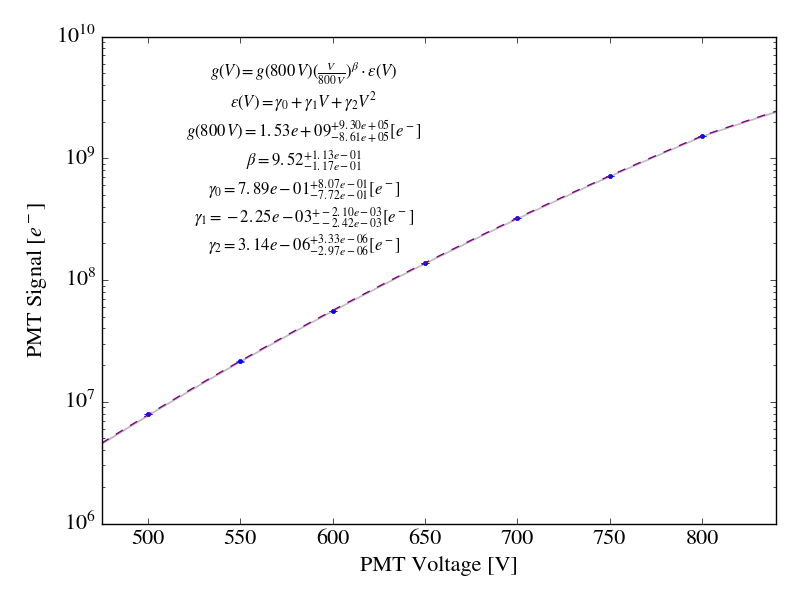
\includegraphics[width=0.49\textwidth]{nerix_mpe_spectrum}
	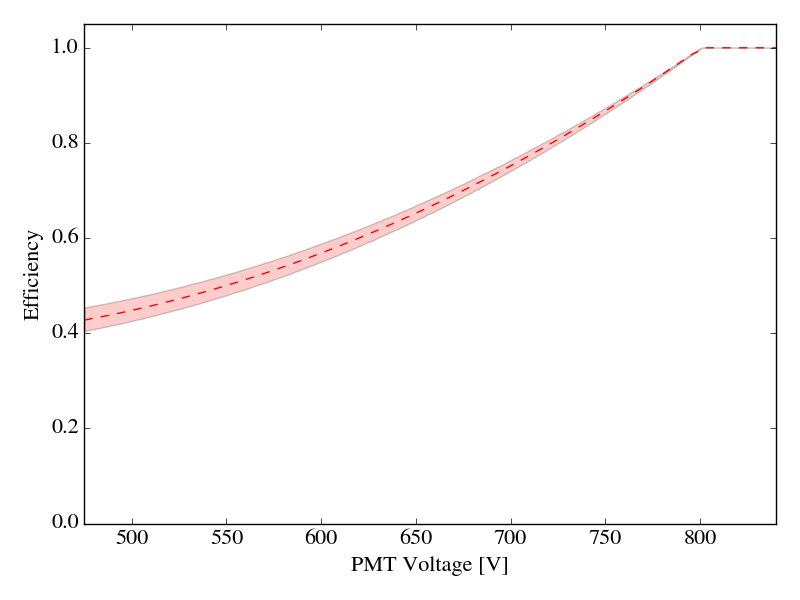
\includegraphics[width=0.49\textwidth]{nerix_collection_efficiency}
	\caption{On the left is the neriX MPE spectrum for the bottom PMT including the collection efficiency function shown on the right.}
	\label{fig:nerix_mpe}
\end{figure}


\subsection{Position Reconstruction and Position Dependence}

Position reconstruction also plays an important role in neriX.  While position reconstruction is not used to remove background events, a fiducial volume is still set to avoid edge effects from field non-uniformity and electrons capturing on the teflon.  Additionally, we do expect a small amount of position dependence for both the S1 and S2.  

To determine the transverse position of the event, we again use the S2 signal seen by the top PMTs.  The four PMTs in the top array actually have four individual anodes that are essentially treated as separate channels --- this means that our four multianode PMTs act as sixteen single anode PMT channels.  While obviously our position reconstruction in the transverse position will be significantly more limited than XENON1T due to the prevalence of edge effects in the small detector and the limited number of pixels, however we can use a neural network trained on an optical simulation of photons produced in between the anode and the gate to estimate the position.  The transverse positions of high-energy ($>40$ PE) nuclear recoils, which should be approximately uniformly distributed in the TPC, at a field of 490 V/cm is shown in the left panel of \figref{fig:nerix_position_reconstruction}.  The small defects in the position reconstruction are likely due to discrepancies in the unmeasured collection efficiencies of the individual PMT channels.

\begin{figure}[t]
        \centering
	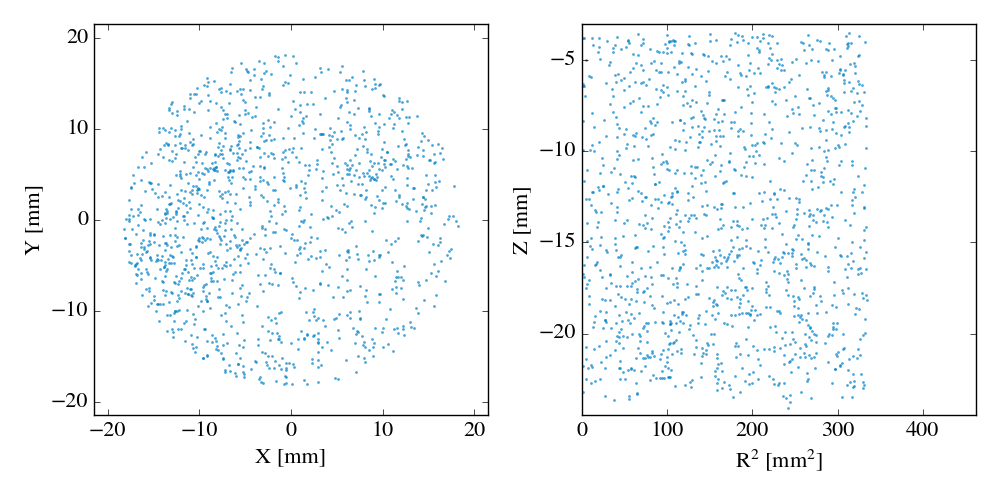
\includegraphics[width=0.99\textwidth]{nerix_position_reconstruction}
	\caption{The spatial distributions of high-energy nuclear recoil events taken at 490 V/cm after fiducial volume and other quality cuts.}
	\label{fig:nerix_position_reconstruction}
\end{figure}

To determine the depth of the interaction, we look at the time between the S1 and S2, also referred to as the \textit{drift time}.  Since the electrons will drift through the liquid xenon at a fixed velocity, this time difference can be used to measure the depth.  The drift velocity in liquid xenon will change as a function of the electric field applied so the drift velocity must be measured for each field used.

To measure the drift velocity, one uses the fact that the scintillation light produced from interactions in the liquid xenon can actually interact with the meshes, releasing electrons in the process.  These photoionization electrons can be seen following large S1s and S2s in waveforms.  Therefore, if one looks at the timing of small S2 signals following a large S1 or S2, one will actually see peaks in the spectrum due to these photoionization electrons, as shown in \figref{fig:nerix_drift_velocity}.  By examining the time distance between the two peaks, we can determine the drift velocity since the distance between the meshes at liquid xenon temperatures is known (23.4 mm).

\begin{figure}[t]
        \centering
	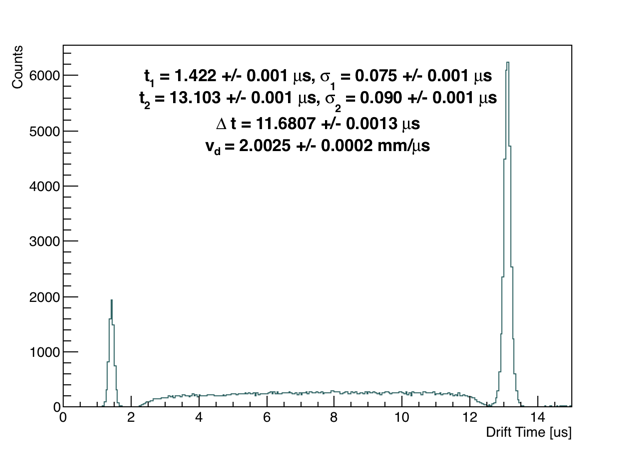
\includegraphics[width=0.8\textwidth]{nerix_drift_velocity}
	\caption{The distribution of small S2s in time after a large S2 at a field of 1020 kV/cm.  Notice the two sharply spike peaks around 1.5 and 13 $\mu$s --- these peaks are due to electrons from the photoionization of the gate and cathode mesh, repectively.  Since we know the distance between these two meshes we can measure the drift velocity at this field.}
	\label{fig:nerix_drift_velocity}
\end{figure}


The drift velocities during this measurement and during the low-energy measurement of the yields of electronic recoils \cite{goetzke2016measurement} are shown in \tabref{tab:nerix_drift_velocities}.  One can see that the drift velocities of all three runs in the detector agree very well with each other (within a few percent).

\begin{table}[b]
\centering
\def\arraystretch{1.3}
\begin{tabular}{cccc}
\hline
Drift Field & 190 V/cm & 490 V/cm & 1020 V/cm \\
\hline
 & \multicolumn{3}{c}{$v_d$ [mm/$\mu$s]} \\
\hline
ER Run 1 & 1.51 & 1.72 & 1.96 \\
ER Run 2 & 1.54 & 1.75 & 1.97 \\
This Work & 1.56 & 1.77 & 2.00 \\
\hline
\end{tabular}
\caption{The measured drift velocities at 190, 490, and 1020 V/cm in neriX for the measurement of the yields of electronic recoils \cite{goetzke2016measurement} and this work.}
\label{tab:nerix_drift_velocities}
\end{table}


While due to the small size of the detector we do not observe a radial dependence of the S1 and S2 signals, we do observe effects due to the depth of the interaction in the detector.  The former effect is caused by the proximity of the interaction to the bottom PMT while the latter effect is caused by electrons drifting to the surface attaching to electronegative impurities.  For more details on each of these effects, please refer to \secref{sec:xe1t_lce_pos_correction} and \secref{sec:xe1t_depth_correction}, respectively.  While not as drastic as the effects in XENON1T, these effects are still on the order of 10--20\% for S1s and 5\% for S2s.  To perform the correction, we use events from the 662 keV peak from \cesium{} and fit the S1 and S2 size as a function of depth.  As expected, we observe the same pattern as XENON1T: events closer to the bottom PMT have larger S1s than those events closer to the liquid-gas interface and events from lower in the detector are more likely to lose charge to impurities in the liquid xenon.  Both of these effects can be seen in \figref{fig:nerix_pos_correction}.  Due to a getter failure, the purification system utilized a getter much further in distance compared to the one used in \citeref{goetzke2016measurement}, leading to a non-negligible electron lifetime.  Both of these effects were monitored over the course of the run and since no discernable time dependence was seen, a run average was taken.


\begin{figure}[t]
        \centering
	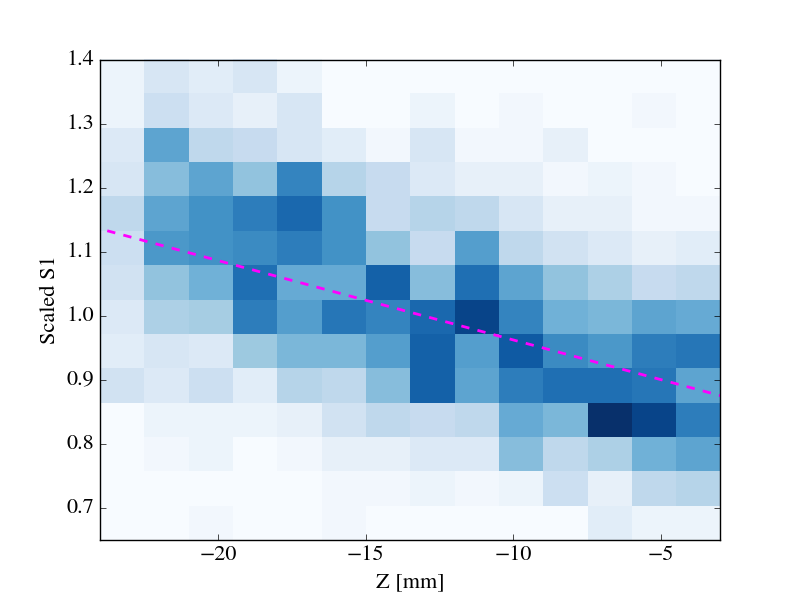
\includegraphics[width=0.45\textwidth]{nerix_s1_z_correction}
	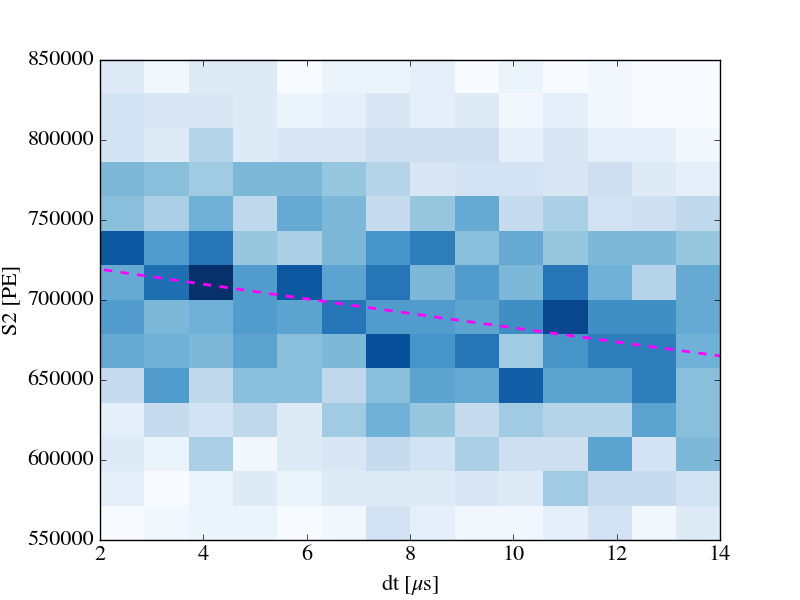
\includegraphics[width=0.45\textwidth]{nerix_s2_dt_correction}
	\caption{The depth correction of the S1 (left) and S2 (right) signals as a function of depth in the detector.}
	\label{fig:nerix_pos_correction}
\end{figure}




\subsection{Single Electron Response}
\label{sec:nerix_gas_gain}

One very important quantity for TPCs that was discussed in chapters two and three is the single electron response (also known as the gas gain).  The single electron response measures how many photoelectrons we expect in our PMTs if a single electron is extracted from the liquid into the gas.  Typically the response is approximated as a Gaussian distribution with a mean, $\mu_G$, and width, $\sigma_G$.  While technically this quantity could be field-dependent due to leakage from the cathode, simulations show that this effect is only on the order of $\sim2\%$ \cite{goetzke2015low}.

We used a source of single electrons already discussed for this calibration: single electrons from the photoionization of the gate.  By using these, we could make a strict time cut rather than search an entire waveform for single electrons which reduces the potential noise.  Even though only the bottom PMT was used for all analyses, the single electron response was fit in two dimensions for extra discrimination power between single and double electron peaks.  A sample fit is shown in \figref{fig:nerix_gas_gain}.  The response of the TPC to single electrons was assumed to be normal for both the top and the bottom PMTs with no correlation.  As in \citeref{aprile2014observation} and \citeref{goetzke2016measurement}, a roll-off was applied at low S2s to represent the loss due to the S2 peak finding efficiency.

\begin{figure}[t]
        \centering
	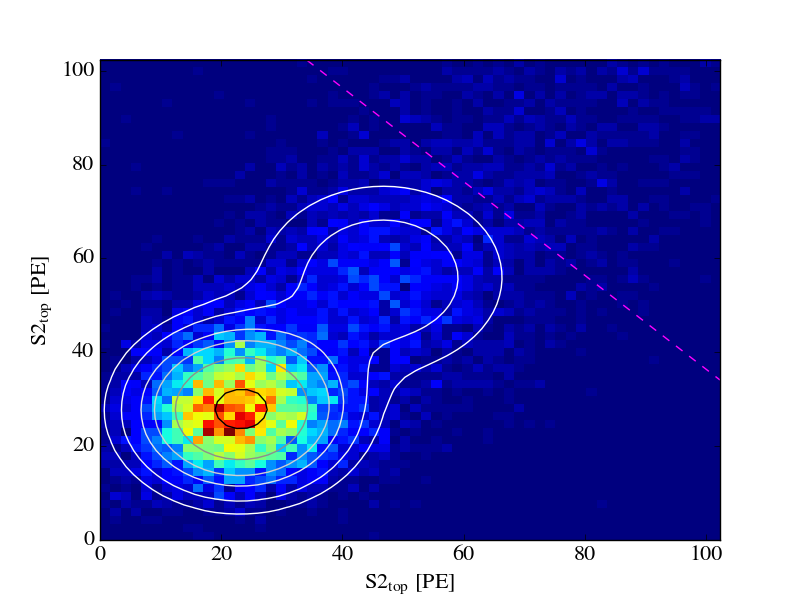
\includegraphics[width=0.85\textwidth]{nerix_gas_gain}
	\caption{The single electron response as measured by the top and bottom PMTs in neriX.  Note that the response, even for a single electron, appears to follow a Gaussian distribution.  The contours show the outline of the fit and the pink line represents the edge of the fit range.}
	\label{fig:nerix_gas_gain}
\end{figure}

As with the position correction, no clear time dependence was observed for the the single electron response so both the mean and width of the distribution were averaged over the course of the run for all fields.



\subsection{Anticorrelation}
\label{sec:nerix_anticorrelation}

As discussed in \secref{sec:lxe_er_observables} and \secref{sec:xe1t_anticorrelation}, due to the lack of quenching factors in electronic recoils the energy of an interaction and the number of photons and free electrons produced are inextricably linked.  This relationship is shown in \eqnref{eqn:nerix_anticorrelation} where $N_q$ is the number of quanta, $\textrm{E}_{\textrm{ER}}$ is the energy of the electronic recoil, $W$ is the average energy required to produce an exciton or electron-ion pair ($13.7 \pm 0.2$ eV \cite{dahl_thesis}), $N_{\gamma}$ is the number of photons produced in the electronic recoil, and $N_e$ is the number of free electrons extracted from the interaction site.

\begin{equation}
        \label{eqn:nerix_anticorrelation}
        N_q = \frac{\textrm{E}_{\textrm{ER}}}{W} = N_{\gamma} + N_{e}
\end{equation} 

In the same way as \secref{sec:xe1t_anticorrelation}, we can put this equation in terms of detector variables including our observables, S1 and S2, the average light collection efficiency, $g_1$, the extraction efficiency, $\eta$, and the mean single electron gain, $G$, as shown in \eqnref{eqn:nerix_anticorrelation_s1_s2}.

\begin{equation}
        \label{eqn:nerix_anticorrelation_s1_s2}
        \frac{\textrm{E}_{\textrm{ER}}}{W} = \frac{\textrm{S1}}{g_1} + \frac{\textrm{S2}}{G \eta}
\end{equation}

This implies that if we have a sample of S1 and S2 signals from a known monoenergetic peak that we can extract the otherwise very difficult to measure quantities $g_1$ and $\eta$.  This type of anticorrelation measurement is typically performed using a single full absorption peak at multiple electric fields (typically done in smaller detectors where the field can be changed easily) or using multiple full absorption peaks from different sources at a single electric field (typically done in larger detectors where electric fields are more difficult to manage and change large amounts).  The latter is done in LUX \cite{akerib2016improved} and XENON1T \cite{aprile2017first}.  For neriX, we decided to vary both to make the measurement as robust as possible: two sources, \cesium{} and \sodium{}, were used to extract monoenergetic events at five different fields.  These events are fit simultaneously to \eqnref{eqn:nerix_anticorrelation_line} where $\textrm{E}_{\textrm{ER}}$ is equal to 662 keV for \cesium{} and 511 keV for \sodium{}.


 \begin{equation}
        \label{eqn:nerix_anticorrelation_line}
        \frac{\textrm{S2}}{\textrm{E}_{\textrm{ER}}} = \frac{G \eta}{g_1} \frac{\textrm{S1}}{\textrm{E}_{\textrm{ER}}} - \frac{G \eta}{W}
\end{equation}

A sample fit is shown in \figref{fig:nerix_anticorrelation}.  No discernable time dependence in the parameters was found and thus a run average was used to describe $g_1$ and $\eta$.

\begin{figure}[t]
        \centering
	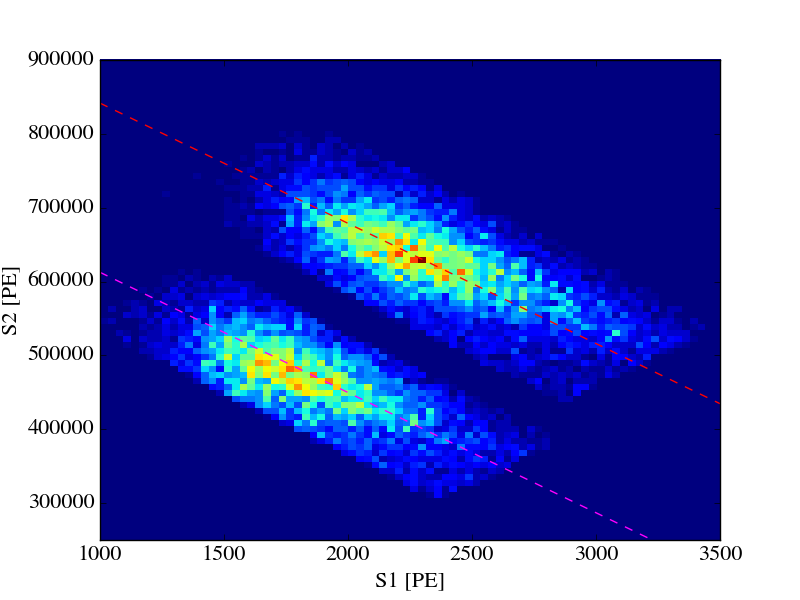
\includegraphics[width=0.85\textwidth]{nerix_anticorrelation}
	\caption{Anticorrelation analysis performed on the full absorption peaks \cesium{} and \sodium{} at five different electric fields.  One can also see the best fit of the model shown overlayed.}
	\label{fig:nerix_anticorrelation}
\end{figure}


\subsection{Trigger Efficiency}
\label{sec:nerix_trig_efficiency}

As discussed in previous chapters the charge yield of nuclear recoils is significantly lower than an equivalent electronic recoil.  Therefore, it is crucial to estimate the efficiency of the trigger as a function of S2 size.  As discussed in \secref{sec:nerix_daq_trigger}, the S2 trigger is actually based on the width of the event however we will use the total S2 size (area) as a proxy to estimate the efficiency.

The measurement of the trigger efficiency is quite simple.  Rather than using the S2 trigger to record events, as is standard for almost all other TPC calibrations, we use a random trigger and digitize the S2 trigger while irradiating the detector with a \sodium{} source.  In this way, we can check each waveform for an S2 and whether or not an S2 trigger was present.  The random trigger ensures that we in no way bias our measurement of the trigger efficiency by requiring that an S2 be present in the waveform.  While this does eliminate the bias, the measurement is very inefficient in terms of storage since many saved waveforms do not contain relevant data.  While ideally one would measure the S2 trigger efficiency regularly, collecting sufficient statistics took approximately three weeks and therefore regular calibrations were impractical.

Once sufficient statistics were collected, one could use large S2 events to find the standard time difference between the S2 peak and the S2 trigger.  With our trigger system, the time difference between the two was 600--800 ns.  With this time cut in place, we could then look at smaller S2 events and determine whether or not a trigger was present.  The results of the measurement are shown in \figref{fig:nerix_trigger_efficiency}.

\begin{figure}[t]
        \centering
	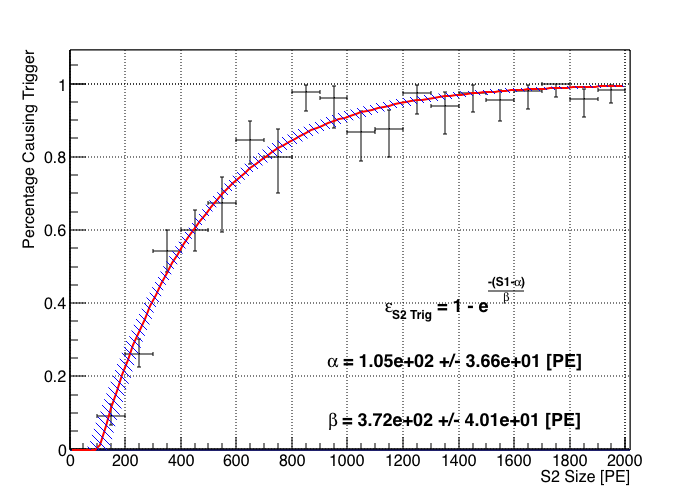
\includegraphics[width=0.85\textwidth]{nerix_trigger_efficiency}
	\caption{The neriX trigger efficiency as measured using a random trigger.  Shown overlaid are the best fit alongside the 68\% credible region.}
	\label{fig:nerix_trigger_efficiency}
\end{figure}



\subsection{Peak Finding Efficiency}
\label{sec:nerix_pf_efficiency}

The second efficiency loss in this measurement is actually on the software side of the analysis.  Once raw data is saved, it is analyzed in a processor where important information is extracted such as the S1 and S2 sizes and locations in the waveform.  While the peak-finding algorithm used to identify S1s and S2s in the waveform is excellent at finding even single electrons (as shown in the single electron response calibration), there is some loss for very small S1 signals.  

Unlike the trigger efficiency, the peak finder's efficiency was not measured directly.  Instead a realistic waveform simulator was developed to study this efficiency loss.  This waveform simulator included effects such as the characteristic pulse shape of the PMT, the noise level in the TPC, and the shape of the S1 signal due to the excimer decay times \cite{hitachi1983effect}.  The waveform simulator was then used to produce events with S1s of known sizes which were then fed into the data processor.  Post-processing, we could then check how many of the S1s in a given range were discovered by the peak finder.  The results of the waveform simulation are shown in \figref{fig:nerix_peak_finder_efficiency}.

\begin{figure}[t]
        \centering
	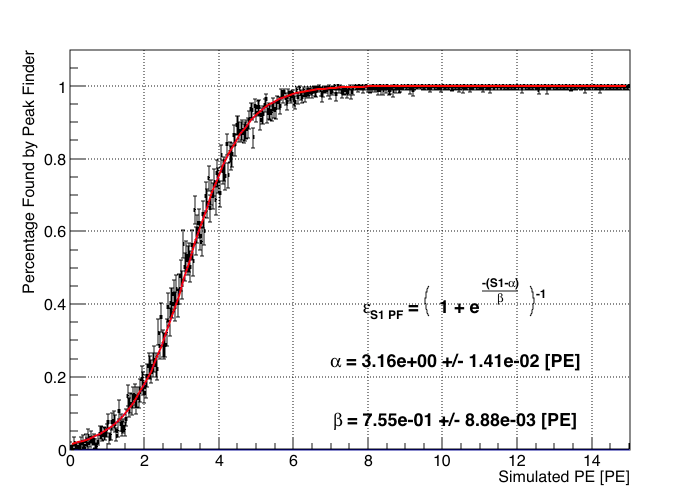
\includegraphics[width=0.85\textwidth]{nerix_peak_finder_efficiency}
	\caption{The neriX peak finding efficiency from empirically based waveform simulations.}
	\label{fig:nerix_peak_finder_efficiency}
\end{figure}





\section{Nuclear Recoil Data Collection}

The data taking run of neriX lasted for approximately four and a half months.  We began collecting coincidence data on March 30, 2016 and completed taking coincidence data on July 4, 2016.  Calibrations and trigger efficiency measurements continued until August 9, 2016 when a power failure occurred overnight resulting in a pressure spike in which xenon was safely released into the pressure relief vessel via the solenoid valve discussed in \secref{sec:nerix_pressure_relief}.

With a total of four M510 liquid scintillator detectors, we were able to measure two scattering angles, and hence energy spectra, simultaneously.  In total, six scattering angles were measured at three different electric fields.  Ultimately, data at the lowest and highest energy were not used: the former due to lack of statistics due the efficiency losses discussed in \secref{sec:nerix_trig_efficiency} and \secref{sec:nerix_pf_efficiency} and the latter due the poor data quality (likely due to the M510 detectors' proximity to the TPC).  On average, it took approximately two weeks to measure two energy setups at a given cathode voltage.

As discussed in \secref{sec:nerix_expt_setup}, we use the positions of the M510 liquid scintillator detectors to restrict the energy spectrum such that it is peaked around a specific energy and does not follow the standard exponentially falling energy spectrum for nuclear recoils in liquid xenon.  The positions of the detectors (and the minitron) were set using an auto-levelling laser mounted on a tripod.  Positions were measured relative to the center of the TPC and marked on the laboratory floor using tape.  The positions of the M510 detectors were chosen such that an energy resolution of 15--25\% was achieved.  \tabref{tab:nerix_ej_positions} shows the positions of the M510 detectors relative to the TPC center\footnote{The minitron was placed at (0, -43.0, 0) cm in the coordinate frame as defined in \tabref{tab:nerix_ej_positions}.}.  The estimated uncertainty in each dimension is 3 mm.


\begin{table}[t]
\centering
\def\arraystretch{1.3}
\begin{tabular}{cc|ccc|ccc}
\hline
$\theta$ & Energy [keV] & \multicolumn{3}{c|}{M510 1 Position [cm]} & \multicolumn{3}{c}{M510 2 Position [cm]} \\
 & & x & y & z & x & y & z \\
\hline
$30^{\circ}$ & $4.95 \pm 0.83$ & 38.1 & 66.4 & -4.6 & -38.3 & 66.4 & 0 \\
$35^{\circ}$ & $6.60 \pm 1.52$ & 24.3 & 34.2 & 0 & -23.9 & 34.2 & -4.6 \\
$45^{\circ}$ & $10.62 \pm 1.54$ & -41.4 & 41.7 & -4.6 & 41.7 & 41.7 & 0 \\
$53^{\circ}$ & $13.95 \pm 2.46$ & 29.5 & 22.3 & 0 & -29.5 & 22.3 & 0 \\
\hline
\end{tabular}
\caption{The positions of the M510 liquid scintillator detectors during coincidence data taking.  The energies and corresponding widths shown are found via a detailed Monte Carlo produced in Geant4 which will be discussed further in \secref{sec:nerix_geant_mc}.}
\label{tab:nerix_ej_positions}
\end{table}

In addition to coincidence data, nuclear recoil data is taken without the coincidence requirement which we refer to as \textit{band data}.  This merely involves replacing the coincidence trigger described in \secref{sec:nerix_daq_trigger} with the S2 hold-off trigger.

A few basic cuts were made to clean the data taken.  The fiducial volume cut was made to ensure the electric field variations were limited to within 20\% and an asymmetry cut, which removes events based on what fraction of the S1 and S2 signals are seen by the top versus bottom PMTs, is made to ensure the removal of noisy events.  For coincidence data, two additional cuts are made based off of the liquid scintillators.  The first selects neutrons in the M510 detectors using the pulse-shape discrimination of the EJ301 liquid scintillator.  The second is a coarse time of flight cut, made using the time difference from the waveform, to ensure that the S1 signal discovered by the peak finder is within 100 ns of the liquid scintillator pulse to remove as many accidental coincidences as possible.  A finer time of flight cut could not be made with a time to amplitude converter (TAC) since our average light collection efficiency is lower than the single phase liquid xenon detectors used to measure the light yield of nuclear recoils in the past \cite{aprile2009new, manzur2010scintillation, plante2011new}\footnote{Technically,  Manzur \textit{et al.} used a dual phase detector operated in a ``single phase'' mode which drastically increased their average light collection efficiency.} and therefore we could not, with high efficiency, use the S1 signal to start the TAC.  %While it would be useful to confirm that our liquid scintillator cut removed almost all of the electronic recoils from neutron activated materials, both \citeref{aprile2009new} (Fig. 4) and \citeref{plante2011new} (Fig. 8) showed that this is the case.

For all data collected, no discernable differences were seen between the individual M510 detectors.  Therefore, all distributions used in the analysis used data from both of the liquid scintillators.  The resulting spectra are shown as a function of both S1 and S2 in \figref{fig:nerix_nr_data_1}, \figref{fig:nerix_nr_data_2}, \figref{fig:nerix_nr_data_3}, and \figref{fig:nerix_nr_data_4}.


\begin{figure}[p]
	\centering
	\includegraphics[width=0.49\textwidth]{../nerix_data_only/{0.345_kV_3000_deg_data_only}.png}
	\includegraphics[width=0.49\textwidth]{../nerix_data_only/{0.345_kV_3500_deg_data_only}.png}

        %\vspace{\floatsep}
        \vspace{0.3cm}

	\centering
	\includegraphics[width=0.49\textwidth]{../nerix_data_only/{0.345_kV_4500_deg_data_only}.png}
	\includegraphics[width=0.49\textwidth]{../nerix_data_only/{0.345_kV_5300_deg_data_only}.png}
	
	\centering
	\caption{Coincidence data taken with a drift field of 190 V/cm.}
	\label{fig:nerix_nr_data_1}
\end{figure}


\begin{figure}[p]
	\centering
	\includegraphics[width=0.49\textwidth]{../nerix_data_only/{1.054_kV_3000_deg_data_only}.png}
	\includegraphics[width=0.49\textwidth]{../nerix_data_only/{1.054_kV_3500_deg_data_only}.png}

        %\vspace{\floatsep}
        \vspace{0.3cm}

	\centering
	\includegraphics[width=0.49\textwidth]{../nerix_data_only/{1.054_kV_4500_deg_data_only}.png}
	\includegraphics[width=0.49\textwidth]{../nerix_data_only/{1.054_kV_5300_deg_data_only}.png}
	
	\centering
	\caption{Coincidence data taken with a drift field of 490 V/cm.}
	\label{fig:nerix_nr_data_2}
\end{figure}


\begin{figure}[p]
	\centering
	\includegraphics[width=0.49\textwidth]{../nerix_data_only/{2.356_kV_3000_deg_data_only}.png}
	\includegraphics[width=0.49\textwidth]{../nerix_data_only/{2.356_kV_3500_deg_data_only}.png}

        %\vspace{\floatsep}
        \vspace{0.3cm}

	\centering
	\includegraphics[width=0.49\textwidth]{../nerix_data_only/{2.356_kV_4500_deg_data_only}.png}
	\includegraphics[width=0.49\textwidth]{../nerix_data_only/{2.356_kV_5300_deg_data_only}.png}
	
	\centering
	\caption{Coincidence data taken with a drift field of 1020 V/cm.}
	\label{fig:nerix_nr_data_3}
\end{figure}


\begin{figure}[p]
	\centering
	\includegraphics[width=0.49\textwidth]{../nerix_data_only/{0.345_kV_-4_deg_data_only}.png}
	\includegraphics[width=0.49\textwidth]{../nerix_data_only/{1.054_kV_-4_deg_data_only}.png}

        %\vspace{\floatsep}
        \vspace{0.3cm}

	\centering
	\includegraphics[width=0.49\textwidth]{../nerix_data_only/{2.356_kV_-4_deg_data_only}.png}

	
	\centering
	\caption{High energy nuclear recoil band data without a coincidence trigger at the three fields measured.}
	\label{fig:nerix_nr_data_4}
\end{figure}



\section{Analysis of Nuclear Recoils in Liquid Xenon}
\label{sec:nerix_analysis}

% need to discuss how previous analyses were done and why light and charge yield do not tell the whole story

As it was stated at the beginning of this chapter, multiple measurements of the response of liquid xenon to nuclear recoils have been made.  However, these previous measurements assumed a simple LXe physics models because they were limited to a single observable\footnote{In some cases, data for both observables was taken but the analysis used only a single observable at a time.}: for each coincidence dataset a single parameter, $\mathcal{L}_{eff}(E_{\textrm{NR}}) = L_y(E_{\textrm{NR}}) / L_y(E_{\textrm{ER}}=122 \, \textrm{keV})$ or $Q_y(E_{\textrm{NR}})$, was used to map the energy to a one-dimensional observable space (S1 or S2) and a generic resolution was applied to account for the widening of the spectrum due to statistical fluctuations in the LXe microphysical process described in \secref{sec:xe_nr_observables}.

While this analysis approach has proved effective, it does have a few underlying issues.  First, this procedure fails to account for correlations between the light and charge that is expected since it only looks at a single observable at a time and therefore we cannot build an effective model for the microphysics of liquid xenon.  Second, the procedure itself is slightly inconsistent --- the same energies in different coincidence spectra have different $\mathcal{L}_{eff}$ applied to them.  Finally, since we are measuring low energies, applying a large smearing term can potentially bias the measurements of the yields at energies close to the efficiency roll-offs.  While the second and third issues can be reduced and carefully controlled, the inability to produce an effective two dimensional observables production model has impacts on the WIMP search, as we saw in \secref{sec:xe1t_wimp_results}.

In this work, a completely new procedure for analyzing nuclear recoil data in xenon was developed.  This procedure was the basis for both the electronic and nuclear recoil calibration of XENON1T (\secref{sec:xe1t_er_nr_calibration}) and the basic framework can be used for all different types of analyses, including the characterization of PMTs which is discussed in \appref{app:pmts}.  This framework, which used GPUs to run a fast Monte Carlo of the model given the parameters under test for likelihood calculations during parameter estimation, allowed us to test and measure light and charge production models for the response of liquid xenon to nuclear recoils for the first time.   

As the procedure followed in \secref{sec:xe1t_er_nr_calibration} was based off of this work, many aspects will be similar.  Therefore, special attention will be specifically devoted to the differences between the two.



\subsection{Monte Carlo Simulation of Energy Spectra}
\label{sec:nerix_geant_mc}


As mentioned during the discussion of the XENON1T nuclear recoil calibration, the first step is to predict the energy spectra you expect to measure.  Even though the energy of the recoil is completely determined by the angle of the scatter, effects from the finite sizes of the detector, nuclear recoils in materials other than the fiducial volume, and accidental coincidences will make the spectra far from monoenergetic.  Therefore, it is necessary to build a detailed Monte Carlo to predict the rate of nuclear recoils at different energies given the experimental setup.

The detailed Monte Carlo for this measurement was done in Geant4 \cite{agostinelli2003geant4}.  The Monte Carlo is built with a realistic description of the neutron generator and its casing and stand, the TPC and the cryostat, the detector support frame, the laboratory floor (for neutron reflections), as well as the measured positions of the M510 liquid scintillator detectors listed in \tabref{tab:nerix_ej_positions}.  Also included in the simulation is the neutron yield as a function of emission angle (shown in \figref{fig:nerix_yield_emission_angle}).

The Geant4 simulation records the track of each particle which includes information about each of the interactions it makes, where they occur, and at what time.  For coincidence data, we are particularly interested in neutrons that elastically scatter in the liquid xenon and the M510 liquid scintillator detectors within a time window defined by our time of flight cut in the data.  For nuclear recoil band data, we only place the condition that a neutron elastically scatters a single time in the fiducial volume with no other requirements.  We cannot require that the neutron does not interact in other materials since this type of cut can, of course, not be made in measured data.  The expected energy spectra for coincidence data and nuclear recoil data without a coincidence requirement are shown in \figref{fig:nerix_mc_energy_spectra}.

There are two striking features of each of the coincidence spectra.  The first is the Gaussian-looking peak around a mean energy --- this peak is due to the exact events we are trying to measure: a single elastic scatter in the liquid xenon and a scatter in the M510 detector.  The width of the peak is almost completely due to the finite sizes of the detector.  The second feature is the near exponential roll-off in energy.  This is due to neutrons that scatter in other materials as well as in the fiducial volume of the TPC.  The energy spectrum expected from nuclear recoils without any coincidence trigger is similar to the expected distribution of events for XENON1T with one critical exception.  In XENON1T, we used an americium-beryllium (AmBe source) that radiates neutrons with energies up to 11 MeV.  The minitron neutron generator, on the other hand, produces near monoenergetic neutrons at an angle of $90^{\circ}$ to the target meaning that our TPC is irradiated with neutrons with an energy very close to 2.45 MeV (for the neutron yield as a function of angle for the minitron please refer to \figref{fig:nerix_yield_emission_angle}).  This implies that there is a maximum energy that can be transferred to a xenon nucleus from neutrons back-scattering.  This maximum energy transfer for 2.45 MeV neutrons on xenon nuclei ranges from 72 to 76 keV depending on which isotope of xenon the neutron interacts with.  This roll-off can clearly be seen in the band energy spectra in \figref{fig:nerix_mc_energy_spectra} but is not present in the spectra from AmBe shown in \figref{fig:xe1t_nr_energy_spec}.



\begin{figure}[t]
        \centering
	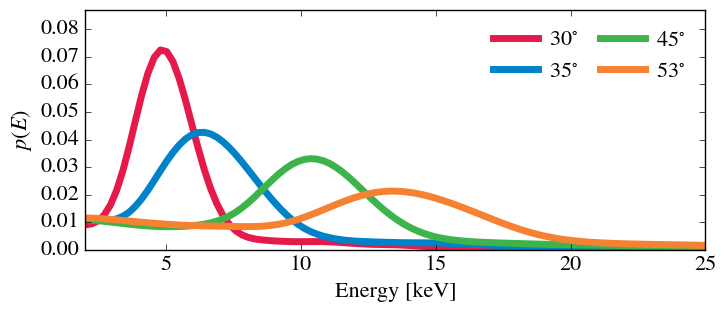
\includegraphics[width=0.99\textwidth]{nerix_energy_spectrum_coin}
	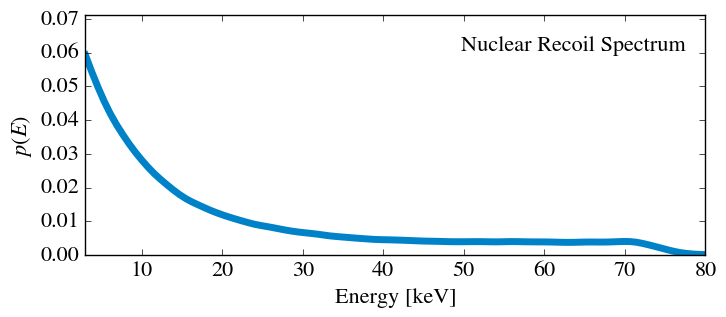
\includegraphics[width=0.99\textwidth]{nerix_energy_spectrum_band}
	\caption{The expected energy spectra for coincidence data (top) and nuclear recoil band data (bottom).  Both of these are used as inputs for the fast Monte Carlo used to estimate the PDF given assumptions on parameters in the signal response model.}
	\label{fig:nerix_mc_energy_spectra}
\end{figure}


\subsection{Light and Charge Production for Nuclear Recoils}
\label{sec:nerix_observables_production}

As discussed in \secref{sec:xe_nr_observables}, recoiling nuclei lose energy via atomic motion that cannot be detected in neriX or other dual-phase TPCs.  We model this loss using Lindhard theory, which gives the energy lost to atomic motion as a function of energy.  This is shown in \eqnref{eqn:nerix_lindhard} in terms of the dimensionless energy $\epsilon$.

\begin{equation}
        \label{eqn:nerix_lindhard}
        \begin{gathered}
                \epsilon = 11.5 \left( \frac{E}{\textrm{keV}} \right) Z^{\sfrac{-7}{3}}, \\
                L(\epsilon) = \frac{k g(\epsilon)}{1 + k g(\epsilon)}, \, \, \, g(\epsilon) = 3 \epsilon^{0.15} + 0.7 \epsilon^{0.6} + \epsilon
        \end{gathered}
\end{equation}

The Lindhard factor, $L$, is then used to approximate the number of quanta as shown in \eqnref{eqn:nerix_nr_quanta}.

\begin{equation}
        \label{eqn:nerix_nr_quanta}
        N_q \sim P \left( \mu = \frac{E \cdot L}{W} \right)
\end{equation}

The choice of the Poisson distribution is the same approximation as used in the XENON1T analysis and is not derived from first principles.  The actual distribution is likely more complicated due to the complex track structure of nuclear recoils in liquid xenon.

With the total number of excitons and ions produced, $N_q$, we can use the exciton-to-ion ratio to simulate the individual numbers of excitons and electron-ion pairs, as shown in \eqnref{eqn:nerix_nr_exciton_ion}.

\begin{equation}
        \label{eqn:nerix_nr_exciton_ion}
        N_{\textrm{ion}} \sim B \left( N=N_q, p = \frac{1}{1 + \frac{N_{\textrm{ex}}}{N_{\textrm{ion}}}} \right) , \, \, \, N_{\textrm{ex}} = N_q - N_{\textrm{ion}}
\end{equation}

We use the same parameterization as \citeref{lenardo2015global} for the exciton-to-ion ratio except that we do not include field dependence, as shown in \eqnref{eqn:nerix_nr_exciton_ion_parameterization}.  Therefore, three constants for the exciton-to-ion ratio are included in the fit to describe each of the three fields.  The energy dependence of the exciton-to-ion ratio, however, is assumed to be the same for all fields.

\begin{equation}
        \label{eqn:nerix_nr_exciton_ion_parameterization}
        \frac{N_{\textrm{ex}}}{N_{\textrm{ion}}}_F = \alpha_F \left( 1 - e^{-\beta \epsilon}  \right)
\end{equation}


With the individual numbers of excitons and ions, we now must consider the possibility of electron-ion pairs recombining to form excitons, resulting in a single photon rather an electron extracted from the site.  Unlike the analysis performed for XENON1T which was dependent on \citeref{lenardo2015global} for the model and priors, we can actually test different parts of the light and charge production model in this analysis.  One aspect of the model tested was the use of the Thomas-Imel model \cite{thomas1987recombination} versus a generic model of recombination.  The generic models tested were polynomials of orders one through five (bounded to a range between zero and one) and a Gompertz function \cite{gompertz1825nature} with and without a constant offset added.  The relative log-likelihoods of the best fits were used to compare the models and it was found that the Thomas-Imel model described the data the best.  Therefore, we define the recombination probability as we did previously.

\begin{equation}
        \label{eqn:nerix_recombination}
        r = 1 - \frac{\textrm{ln}(1 + N_{ion} \sigma_F)}{N_{ion} \sigma_F}
\end{equation}

Unlike \citeref{lenardo2015global}, though, we do not parameterize the field dependence of $\sigma$ and instead keep three $\sigma$ parameters included in the fit: one used at each field.  In this way, no assumptions about the field dependence of recombination were made.  

The recombination probability was used in the same way as before to simulate the number of electron-ion pairs that recombine.


\begin{equation}
        \label{eqn:xe1t_nr_recombination}
        \begin{gathered}
                N_{\textrm{rec}} \sim B(N = N_{\textrm{ion}}, p = r), \\ 
                N_{\textrm{ion}} \leftarrow N_{\textrm{ion}} - N_{\textrm{rec}}, \, \, \,  N_{\textrm{ex}} \leftarrow N_{\textrm{ex}} + N_{\textrm{rec}}
        \end{gathered}
\end{equation}


Finally, we consider biexcitonic quenching, which results from the collision of two excitons.  We estimate this quenching using Birk's saturation law, as shown in \eqnref{eqn:nerix_birks_quenching}, since one would expect that the density of excitons in the track is proportional to the electronic stopping power \cite{mei2008model, tretyak2010semi, bezrukov2011interplay}.


\begin{equation}
        \label{eqn:nerix_birks_quenching}
        f_B = \frac{1}{1 + a \frac{dE}{dx}} = \frac{1}{1 + \eta \epsilon^{- \sfrac{1}{2}}}
\end{equation}


We choose to follow the treatment of \citeref{akerib2016low} and fix the energy dependence of the stopping power, as seen in \eqnref{eqn:nerix_birks_quenching}.  This is different than the treatment in the XENON1T analysis which was based off of the model in \citeref{lenardo2015global} and was chosen because track simulations see this sort of energy dependence up to a few hundred keV and to prevent the possibility of overfitting at the high-energy end of the nuclear recoil spectrum.

In summary, there are nine free parameters in the liquid xenon model: $k$, a constant relating the electronic stopping power to the velocity, $\alpha_F$, the exciton-to-ion ratio at each of the three fields, $\beta$, the energy dependence of the exciton-to-ion ratio, $\sigma_F$, the recombination constant at each of the three fields, and $\eta$, Birk's constant for liquid xenon.  No priors outside of physical restrictions (all parameters greater than zero) are used.



\subsection{Detector Model for Signal Production}

While the major steps of the detector model are the same as for XENON1T, since the TPCs operate in identical ways, several simplifications to the detector response model could be made such as the exclusion of position corrections.  


\subsubsection{Detection of Scintillation Photons}


To begin the detector physics model, we consider the average light collection efficiency that was measured via the anticorrelation calibration discussed in \secref{sec:nerix_anticorrelation}.  As in the XENON1T model, we also consider double photoelectron emissions \cite{faham2015measurements} since the scintillation light has a wavelength of 178 nm.  However, we do not consider effects due to the position of the interaction in the detector.  The number of photons producing at least a single photoelectron, $N_i$, is simulated by \eqnref{eqn:nerix_binomial_lce} in the fast Monte Carlo.


\begin{equation}
        \label{eqn:nerix_binomial_lce}
        \begin{gathered}
                N_{\textrm{i}} \sim B \left( N = N_{\gamma}, p = \frac{g_1}{1 + p_{\textrm{DPE}}} \right), \\
                %N_{\textrm{pe}} \leftarrow N_{\textrm{pe}} + B(N=N_{\textrm{pe}}, p=p_{\textrm{DPE}})
        \end{gathered}
\end{equation}


With the number of photons causing at least a single photoelectron, we can account for how many photoelectrons were produced in total again using the probability for double photoelectron emission.


\begin{equation}
        N_{\textrm{PE}} \sim N_{\textrm{i}} + B(N=N_{\textrm{i}}, p=p_{\textrm{DPE}})
\end{equation}

We now apply a smearing on the size of the S1 PMT signal according to the measured resolution of the bottom PMT of the TPC.  Note that we do not use the cascade model to simulate the charge distribution from the PMT due to simulation time constraints and instead approximate the response with a normal distribution.

\begin{equation}
        \textrm{S1}' \sim N \left( \mu=N_{\textrm{PE}}, \sigma^2=R^2 \cdot N_{\textrm{PE}} \right)
\end{equation}

With an approximation of the charge signal output by the PMT, we can consider processor effects.  First, a probability of the processor finding the S1, $p_{\textrm{PF}}$,  is determined using the size of the signal and the efficiency curve determined via the simulation discussed in \secref{sec:nerix_pf_efficiency}.    

We then apply a smearing to mainly capture the non-zero resolution of the processor reconstruction but also effects due to noise, position dependence of the light collection efficiency, and time variation of detector parameters.  We assume that effects due to processor reconstruction should diminish as a function of the S1 signal size (this assumption was corroborated via the waveform simulator) and the other effects should be independent of signal size.  The functional form of the generic smearing is shown in \eqnref{eqn:nerix_s1_smearing}.


\begin{equation}
        \label{eqn:nerix_s1_smearing}
        \begin{gathered}
                \sigma_{\textrm{S1}} = a_{\textrm{S1}} + b_{\textrm{S1}} \cdot e^{\sfrac{-\textrm{S1}}{c_{\textrm{S1}}}} \\
                \textrm{S1} \sim N \left( \mu = \textrm{S1}', \sigma^2  = \sigma_{\textrm{S1}}^2 \right)
        \end{gathered}
\end{equation}

Since no position dependent effects are considered, the S1 from \eqnref{eqn:nerix_s1_smearing} can be matched to the corrected S1 data.


\subsubsection{Detection of Electrons}


We do not consider effects from the electron lifetime of the detector in the fast Monte Carlo of neriX since it is much larger than the maximum drift time of electrons in the TPC and since we compare to corrected data.  We assume that all electrons reach the liquid surface where they have a probability of extraction into the gas, $p_{\textrm{extracted}}$.


\begin{equation}
        \label{eqn:nerix_binomial_ee}
        N_{\textrm{extracted}} \sim B \left( N= N_{\textrm{L-G Interface}}, p=p_{\textrm{extracted}} \right)
\end{equation}


With the number of electrons extracted from the gas, we can next account for excitation caused by these electrons in the gaseous xenon as well as the smearing due to the PMTs.  We approximate the number of photoelectrons detected in this secondary amplification as a Gaussian process as shown in \eqnref{eqn:nerix_gas_gain} where $G$ is the mean number of photoelectrons detected for a single extracted electron, $\sigma_G$ is the width of the photoelectron distribution for a single extracted electron, both of which are measured in the calibration described in \secref{sec:nerix_gas_gain}, and $N_{\textrm{PE}}$ is the number of photoelectrons digitized after smearing from the PMTs.

\begin{equation}
        \label{eqn:nerix_gas_gain}
        N_{\textrm{PE}} \sim N(\mu=G , \sigma^2=\sigma_G^2)
\end{equation}


With an approximation of the charge signal output by the PMT for the S2, we can consider the probability of a signal of a given size causing a trigger such that the event is digitized and saved.  To determine this probability, $p_{\textrm{Trigger}}$, we simply input the S2 signal size into the curve measured in the trigger efficiency calibration discussed in \secref{sec:nerix_trig_efficiency}.

The final step in the fast Monte Carlo for the S2 of an event is to apply a smearing term in the same way as the S1 to cover effects such as processor reconstruction, electron lifetime, and the variation of detector parameters in time (such as the gas gain).  The functional form of this generic smearing, shown in \eqnref{eqn:nerix_s2_smearing}, is the same as the form used for the S1.


\begin{equation}
        \label{eqn:nerix_s2_smearing}
        \begin{gathered}
                \sigma_{\textrm{S2}} = a_{\textrm{S2}} + b_{\textrm{S2}} \cdot e^{\sfrac{-\textrm{S2}}{c_{\textrm{S2}}}} \\
                \textrm{S2} \sim N \left( \mu = N_{\textrm{PE}}, \sigma^2  = \sigma_{\textrm{S2}}^2 \right)
        \end{gathered}
\end{equation}


The peak-finding and processor efficiency are combined such that the weight of the event in the histogram that is used to compare the model with the given parameters to data is $w = p_{\textrm{PF}} \cdot p_{\textrm{Trigger}}$.



\subsection{Energy Inputs for Fast Monte Carlo}


Of course the first ingredient for the fast Monte Carlo is the energy spectra.  For nuclear recoil band data (no coincidence requirement), we simply input the expected nuclear recoil spectrum, shown in \figref{fig:nerix_mc_energy_spectra}, given our experimental setup.  For coincidence data, we of course use the expected energy spectra, also shown in \figref{fig:nerix_mc_energy_spectra}, but we must also consider the potential for accidental coincidences between nuclear recoils in the TPC and nuclear recoils in the liquid scintillator since we do not have a fine time-of-flight cut.  In this analysis, we use the nuclear recoil band energy spectrum as the accidental coincidence energy spectrum.  To estimate this background in the data, we introduce an additional parameter into the fit, $p_{\textrm{acc}}$, that defines the probability that the event simulated is from the accidental coincidence spectrum rather than the true coincidence spectrum.  This parameter is unique to each coincidence dataset since the accidental coincidence rate is dependent on the location of the M510 liquid scintillator detectors and on the minitron neutron generator rate, which was not fixed even for data collected with the M510 detectors in the same position (e.g., $35^{\circ}$ data taken at two different electric fields).



\subsection{Posterior Estimation}


The posterior estimation procedure is almost identical to the one outlined for XENON1T in \secref{sec:xe1t_mc_likelihood} and \secref{sec:xe1t_mcmc} with only a minor modification since we have fifteen spectra for fitting.  

As in the XENON1T analysis, we use a binned likelihood to compare the data spectra and Monte Carlo spectra.  However, unlike all previous fixed-angle measurements, we analyze all of the datasets simultaneously to maximize the amount of information used since many parameters are shared between some or all datasets (e.g., $k$ is shared between all datasets while the recombination constant $\sigma_F$ is only shared between datasets taken with the same electric field.  While this is a more ambitious approach, it does have costs in terms of the time required to estimate the posterior since this will increase the dimension of the posterior space and the required time for parameter estimation goes as $\mathcal{O}(d^2)$.  Therefore, our likelihood is given by \eqnref{eqn:nerix_binned_likelihood} where $i$ is the index of the bins and $j$ is the index of the dataset.


\begin{equation}
        \label{eqn:nerix_binned_likelihood}
        \begin{gathered}
                \mathcal{L}_{i,j} = \frac{\hat{b}_{i,j}^{b_{i,j}} e^{-\hat{b}_{i,j}}}{b_{i,j}!} \implies \mathcal{L} = \prod_j \prod_i \mathcal{L}_{i,j} \\ 
                ln(\mathcal{L}) = \sum_j \sum_i ln(\mathcal{L}_{i,j}) = \sum_j \sum_i ( b_{i,j} ln(\hat{b}_{i,j}) - \hat{b}_{i,j} - ln(b_{i,j}!) )
        \end{gathered}
\end{equation}


In this analysis, as in the analysis performed for XENON1T, the affine-invariant implementation of a Markov Chain Monte Carlo (MCMC) was used to sample from the posterior.  For a brief summary on MCMCs, please refer to \secref{sec:xe1t_mcmc}.  The priors used were based on the independent calibrations discussed in \secref{sec:nerix_cals} and physical constraints.

Due to the random nature of the fast Monte Carlo simulation used to estimate the PDF in observables space given the parameter, we expect fluctuations in the log-likelihood.  These fluctuations do not effect the outcome of the parameter estimation however they do slow down convergence.  To speed up convergence, one can artificially suppress the log-likelihood but this has the effect of widening the posterior compared to an unsuppressed version of the log-likelihood\cite{anthony2017characterization}.  In this work, we decided to suppress the log-likelihood by a factor of 10 such that fits could be done on a reasonable time-scale and so systematic studies could be performed.  This implies that the results shown could have been improved by increasing the number of fast Monte Carlo events used to estimate the PDF or by allowing the parameter estimation to run for a longer amount of time without suppression. 


\subsection{Results}
\label{sec:nerix_results}

All fifteen datasets were fit simultaneously using a server optimized for this type of analysis, designed by the author.  The most important feature of the server relevant for this analysis are the six GPU cards that can be used in parallel to provide further increases in speed beyond the CPU versus GPU gap discussed in \appref{app:gpus}.  The full estimation of the posterior takes approximately 1.5 weeks of 24 hour run time on five of the GPUs.


The results of parameter estimation are shown with the data in \figref{fig:nerix_nr_best_fit_1}, \figref{fig:nerix_nr_best_fit_2}, \figref{fig:nerix_nr_best_fit_3}, and \figref{fig:nerix_nr_best_fit_4}.  For the one-dimensional plots, the data is overlaid by the best-fit result and the 68\% credible region of the fit.  %The credible region is made by randomly drawing sets of parameters from the posterior and taking the $\pm 1 \sigma$ range for each bin in the histogram.

%While the majority of the datasets agree well with the model visually, there are a few that appear to disagree.  This same trend is seen when quantitatively evaluating the quality of our fits via the Peacock-Fasano-Francheschini test.  The Peacock-Fasano-Francheschini test is a two dimensional unbinned goodness of fit test analogous to the Kolmogorov-Smirnov test in one dimension.  The Peacock-Fasano-Francheschini test looks for the quadrant around a datapoint where the observed and expected fraction of events disagrees most --- the largest discrepancy observed becomes the test statistic.  By bootstrapping data and Monte Carlo, we can use this test statistics to give us a p-value for the fit \cite{peacock1983two, fasano1987multidimensional}.  These p-values are shown in \tabref{tab:nerix_pvalues}.


One can see visually that our data agrees quite well with the model within the statistical uncertainty.  The Peacock-Fasano-Francheschini test, whose results are shown in \tabref{tab:nerix_pvalues}, does seem to indicate a potential issue with the 10 keV ($45^{\circ}$) data however one should note that this test does not account for the uncertainty in our parameter estimation and only uses the best-fit parameters.  One can also notice a slight mismatch at low S2 values --- we believe that this is due to anomalous background events where the neutron scatters once in the fiducial volume and another time below the cathode or very close to the wall, where the charge of the interaction cannot be collected.  These types of interactions would be indistinguishable from single scatters (since we cannot resolve the time difference between the S1 signals) and would cause disagreements below the nuclear recoil band (since the S2 would be smaller relative to the expected S1).  We believe that the width of the S2 distribution was artificially expanded via the generic S2 smearing function to try to account for these events that are not included in the simulation.






\begin{figure}[p]
	\centering
	

	\includegraphics[width=0.42\textwidth]{../nerix_best_fits/{0.345_kV_3000_deg_s1_2d_thesis}.png}
	\includegraphics[width=0.42\textwidth]{../nerix_best_fits/{0.345_kV_3500_deg_s1_2d_thesis}.png}
	        
	\includegraphics[width=0.42\textwidth]{../nerix_best_fits/{0.345_kV_3000_deg_s2_thesis}.png}
	\includegraphics[width=0.42\textwidth]{../nerix_best_fits/{0.345_kV_3500_deg_s2_thesis}.png}


        %\vspace{\floatsep}
        \vspace{1.5cm}

	\centering
	
	\includegraphics[width=0.42\textwidth]{../nerix_best_fits/{0.345_kV_4500_deg_s1_2d_thesis}.png}
	\includegraphics[width=0.42\textwidth]{../nerix_best_fits/{0.345_kV_5300_deg_s1_2d_thesis}.png}
	        
	\includegraphics[width=0.42\textwidth]{../nerix_best_fits/{0.345_kV_4500_deg_s2_thesis}.png}
	\includegraphics[width=0.42\textwidth]{../nerix_best_fits/{0.345_kV_5300_deg_s2_thesis}.png}
	
	\centering
	\caption{Coincidence data taken with a drift field of 190 V/cm compared to Monte Carlo generated spectra.  From top to bottom: data in two-dimensions, the best-fit results in two dimensions, data projected into S1 space overlaid with the best-fit model and 68\% credible region, and data projected into S2 space in different S1 regions overlaid with the best-fit model and 68\% credible region.}
	\label{fig:nerix_nr_best_fit_1}
\end{figure}


\begin{figure}[p]
	\centering
	

	\includegraphics[width=0.42\textwidth]{../nerix_best_fits/{1.054_kV_3000_deg_s1_2d_thesis}.png}
	\includegraphics[width=0.42\textwidth]{../nerix_best_fits/{1.054_kV_3500_deg_s1_2d_thesis}.png}
	        
	\includegraphics[width=0.42\textwidth]{../nerix_best_fits/{1.054_kV_3000_deg_s2_thesis}.png}
	\includegraphics[width=0.42\textwidth]{../nerix_best_fits/{1.054_kV_3500_deg_s2_thesis}.png}


        %\vspace{\floatsep}
        \vspace{1.5cm}

	\centering
	
	\includegraphics[width=0.42\textwidth]{../nerix_best_fits/{1.054_kV_4500_deg_s1_2d_thesis}.png}
	\includegraphics[width=0.42\textwidth]{../nerix_best_fits/{1.054_kV_5300_deg_s1_2d_thesis}.png}
	        
	\includegraphics[width=0.42\textwidth]{../nerix_best_fits/{1.054_kV_4500_deg_s2_thesis}.png}
	\includegraphics[width=0.42\textwidth]{../nerix_best_fits/{1.054_kV_5300_deg_s2_thesis}.png}
	
	\centering
	\caption{Coincidence data taken with a drift field of 490 V/cm compared to Monte Carlo generated spectra.  From top to bottom: data in two-dimensions, the best-fit results in two dimensions, data projected into S1 space overlaid with the best-fit model and 68\% credible region, and data projected into S2 space in different S1 regions overlaid with the best-fit model and 68\% credible region.}
	\label{fig:nerix_nr_best_fit_2}
\end{figure}


\begin{figure}[p]
	\centering
	

	\includegraphics[width=0.42\textwidth]{../nerix_best_fits/{2.356_kV_3000_deg_s1_2d_thesis}.png}
	\includegraphics[width=0.42\textwidth]{../nerix_best_fits/{2.356_kV_3500_deg_s1_2d_thesis}.png}
	        
	\includegraphics[width=0.42\textwidth]{../nerix_best_fits/{2.356_kV_3000_deg_s2_thesis}.png}
	\includegraphics[width=0.42\textwidth]{../nerix_best_fits/{2.356_kV_3500_deg_s2_thesis}.png}


        %\vspace{\floatsep}
        \vspace{1.5cm}

	\centering
	
	\includegraphics[width=0.42\textwidth]{../nerix_best_fits/{2.356_kV_4500_deg_s1_2d_thesis}.png}
	\includegraphics[width=0.42\textwidth]{../nerix_best_fits/{2.356_kV_5300_deg_s1_2d_thesis}.png}
	        
	\includegraphics[width=0.42\textwidth]{../nerix_best_fits/{2.356_kV_4500_deg_s2_thesis}.png}
	\includegraphics[width=0.42\textwidth]{../nerix_best_fits/{2.356_kV_5300_deg_s2_thesis}.png}
	
	\centering
	\caption{Coincidence data taken with a drift field of 1020 V/cm compared to Monte Carlo generated spectra.  From top to bottom: data in two-dimensions, the best-fit results in two dimensions, data projected into S1 space overlaid with the best-fit model and 68\% credible region, and data projected into S2 space in different S1 regions overlaid with the best-fit model and 68\% credible region.}
	\label{fig:nerix_nr_best_fit_3}
\end{figure}


\begin{figure}[p]
	\centering
	

	\includegraphics[width=0.42\textwidth]{../nerix_best_fits/{0.345_kV_-4_deg_s1_2d_thesis}.png}
	\includegraphics[width=0.42\textwidth]{../nerix_best_fits/{1.054_kV_-4_deg_s1_2d_thesis}.png}
	        
	\includegraphics[width=0.42\textwidth]{../nerix_best_fits/{0.345_kV_-4_deg_s2_thesis}.png}
	\includegraphics[width=0.42\textwidth]{../nerix_best_fits/{1.054_kV_-4_deg_s2_thesis}.png}


        %\vspace{\floatsep}
        \vspace{1.5cm}

	\centering
	
	\includegraphics[width=0.42\textwidth]{../nerix_best_fits/{2.356_kV_-4_deg_s1_2d_thesis}.png}\\
	\includegraphics[width=0.42\textwidth]{../nerix_best_fits/{2.356_kV_-4_deg_s2_thesis}.png}
	        
	
	\centering
	\caption{The high-energy nuclear recoil band data at all three fields compared to Monte Carlo generated spectra.  From top to bottom: data in two-dimensions, the best-fit results in two dimensions, data projected into S1 space overlaid with the best-fit model and 68\% credible region, and data projected into S2 space in different S1 regions overlaid with the best-fit model and 68\% credible region.}
	\label{fig:nerix_nr_best_fit_4}
\end{figure}



\begin{table}[p]
\centering
\def\arraystretch{1.22}
\begin{tabular}{c|ccccc}
 & NR Band & 5 keV & 7 keV & 10 keV & 15 keV \\
\hline
190 V/cm & 0.227 & 0.241 & 0.188 & 0.017 & 0.392 \\
490 V/cm & 0.036 & 0.120 & 0.157 & 0.011 & 0.376 \\
1020 V/cm & 0.080 & 0.249 & 0.186 & 0.054 & 0.412 \\
\end{tabular}
\caption{The estimated p-values of the best-fit model calculated using the Peacock-Fasano-Francheschini test statistic.}
\label{tab:nerix_pvalues}



\centering
\def\arraystretch{1.22}
\begin{tabular}{c|cc}
Parameter & Result & Prior \\
\hline
$w$ [eV] & $13.7 \pm 0.2$ & $13.7 \pm 0.2$ \\
$k$ & $0.188^{+0.008}_{-0.007}$ & - \\
$\beta$ & $2650^{+1690}_{-1590}$ & - \\
$\sigma_{\textrm{190 V/cm}}$ & $0.00837 \pm 0.00014$ & - \\
$\sigma_{\textrm{490 V/cm}}$ & $0.00864^{+0.00047}_{-0.00041}$ & - \\
$\sigma_{\textrm{1020 V/cm}}$ & $0.00904^{+0.00046}_{-0.00040}$ & - \\
$\alpha_{\textrm{190 V/cm}}$ & $1.10 \pm 0.06$ & - \\
$\alpha_{\textrm{490 V/cm}}$ & $1.07^{+0.07}_{-0.05}$ & - \\
$\alpha_{\textrm{1020 V/cm}}$ & $0.99 \pm 0.05$ & - \\
$\eta$ & $1.85^{+0.27}_{-0.26}$ & - \\
\end{tabular}
\caption{The median of the marginalized posterior for each parameter in the light and charge production model along with $16^{\textrm{th}}$ and $84^{\textrm{th}}$ percentiles.}
\label{tab:nerix_physical_model}



\centering
\def\arraystretch{1.22}
\begin{tabular}{cc|c}
Field [V/cm] & Angle & Probability of Accidental Coincidence \\
\hline
190 & $30^{\circ}$ & $0.309^{+0.135}_{-0.123}$ \\
190 & $35^{\circ}$ & $0.117^{+0.131}_{-0.083}$ \\
190 & $45^{\circ}$ & $0.401^{+0.227}_{-0.238}$ \\
190 & $53^{\circ}$ & $0.169^{+0.123}_{-0.108}$ \\

490 & $30^{\circ}$ & $0.359^{+0.133}_{-0.124}$ \\
490 & $35^{\circ}$ & $0.125^{+0.116}_{-0.086}$ \\
490 & $45^{\circ}$ & $0.283^{+0.195}_{-0.178}$ \\
490 & $53^{\circ}$ & $0.189^{+0.138}_{-0.121}$ \\

1020 & $30^{\circ}$ & $0.384^{+0.150}_{-0.154}$ \\
1020 & $35^{\circ}$ & $0.108^{+0.115}_{-0.071}$ \\
1020 & $45^{\circ}$ & $0.364^{+0.247}_{-0.203}$ \\
1020 & $53^{\circ}$ & $0.264^{+0.109}_{-0.113}$ \\

\end{tabular}
\caption{The median of the marginalized posterior for the accidental coincidence background probabilities along with $16^{\textrm{th}}$ and $84^{\textrm{th}}$ percentiles.}
\label{tab:nerix_bkg_prob}



\end{table}



% to make high stat version of MC remember change number of steps to 1 to save time (takes best fit so doesn't matter)


The marginalized results of parameter estimation are shown in \tabref{tab:nerix_physical_model} for the parameters of microphysics model and in \tabref{tab:nerix_detector_model} for the parameters of the detector model.  The background probabilities measured are shown in \tabref{tab:nerix_bkg_prob}.  A flattened form of the posterior is shown in \figref{fig:nerix_physical_corner} for the parameters of the light and charge production model.  


%\begin{table}[t]

%\end{table}



\begin{table}[t]
\centering
\def\arraystretch{1.3}
\begin{tabular}{c|cc}
Parameter & Result & Prior \\
\hline
$g_1$ [PE/$\gamma$] & $0.125 \pm 0.001$ & $0.125 \pm 0.003$  \\
$R_{\textrm{SPE}}$ & $0.645 \pm 0.006$ & $0.644 \pm 0.006$ \\
$p_{\textrm{extracted}}$ & $0.905^{+0.024}_{-0.027}$ & $0.903 \pm 0.028$ \\
$G$ [PE] & $22.9 \pm 0.6$ & $22.9 \pm 0.6$  \\
$\sigma_G$ [PE] & $8.59^{+0.33}_{-0.31}$ & $8.62 \pm 0.31$  \\
$p_{\textrm{DPE}}$ & $0.205^{+0.023}_{-0.024}$ & $0.17 - 0.24$ \\

$\alpha_{\textrm{S1}}$ [PE] & $3.16 \pm 0.01$ & $3.16 \pm 0.01$ \\
$\beta_{\textrm{S1}}$ [PE] & $0.754^{+0.010}_{-0.009}$ & $0.755 \pm 0.009$ \\

$\alpha_{\textrm{S2}}$ [PE] & $117 \pm 28$ & $114 \pm 28$ \\
$\beta_{\textrm{S2}}$ [PE] & $374^{+33}_{-36}$ & $382 \pm 34$ \\

$a_{\textrm{S1}}$ & $0.185^{+0.014}_{-0.015}$ & - \\
$b_{\textrm{S1}}$ & $2.76^{+5.62}_{-2.12}$ & - \\
$c_{\textrm{S1}}$ & $0.514^{+0.624}_{-0.357}$ & - \\

$a_{\textrm{S2}}$ & $0.0955^{+0.0141}_{-0.0152}$ & - \\
$b_{\textrm{S2}}$ & $0.509^{+0.156}_{-0.123}$ & - \\
$c_{\textrm{S2}}$ & $658^{+208}_{-121}$ & - \\

\end{tabular}
\caption{The median of the marginalized posterior for each parameter in detctor model along with $16^{\textrm{th}}$ and $84^{\textrm{th}}$ percentiles.  $\alpha_{\textrm{S1}}$ and $\beta_{\textrm{S1}}$ are the parameters for peak finding efficiency, whose functional form is shown in \figref{fig:nerix_peak_finder_efficiency}, while $\alpha_{\textrm{S2}}$ and $\beta_{\textrm{S2}}$ are the parameters of the trigger efficiency, whose functional form is shown in \figref{fig:nerix_trigger_efficiency}.  The parameters $a$, $b$, and $c$ are for the generic S1 and S2 smearing functions described by \eqnref{eqn:nerix_s1_smearing} and \eqnref{eqn:nerix_s2_smearing}.}
\label{tab:nerix_detector_model}
\end{table}



%\begin{table}[t]

%\end{table}


\begin{figure}[t]
        \centering
	\includegraphics[width=0.85\textwidth]{corner_plot_physical_pars}
	\caption{Our estimate of the posterior for the light and charge production model from the MCMC.}
	\label{fig:nerix_physical_corner}
\end{figure}


To compare this work with previous measurements, we plot the light and charge yield predicted by our model with the 68\% credible region alongside recent studies that measured either the light or charge yield in \figref{fig:nerix_ly_qy}.  Also included in \figref{fig:nerix_ly_qy} are our measurements of $L_y$ and $Q_y$ using the traditional method described at the beginning of \secref{sec:nerix_analysis}.   One striking feature of the yields is that this work found no statistically significant difference in the yields at the fields used at all energies.  This supports the results of \citeref{aprile2006simultaneous} and \citeref{manzur2010scintillation} which only measured the effect above $\sim 45$ keV.  Also of note is the slight disagreement in results when using a physical model (band) versus the traditional model where a single light and charge yield, along with generic smearing terms, are used  (points).   In this analysis, the disagreement is likely due to the close proximity of the liquid scintillator detectors to neriX, which broadens the expected energy spectrum, relative to \citeref{plante2011new}.  However, for this reason, future fixed-angle scattering measurements should consider this effect in their analysis and attempt to avoid this potential bias completely by utilizing a more physically motivated model.



\begin{figure}[p]
        \centering
	\includegraphics[width=0.8\textwidth]{nerix_ly_qy}
	\caption{Measured light and charge yields in this work (red, green, and blue band) compared with previous measurements \cite{aprile2005scintillation,aprile2006simultaneous,sorensen2009scintillation,aprile2009new,manzur2010scintillation,horn2011nuclear,plante2011new, aprile2013response,akerib2016low}.  The red, green, and blue bands are the results from using the physical observables model while the points come from the matching technique used in previous fixed-angle scattering measurements.  The reference line is the best-fit global result from \citeref{lenardo2015global} at 490 V/cm.  An energy cutoff of 3 keV is chosen as this represents an approximately 10\% detection efficiency assuming a light yield of 5.5 photons/keV and charge yield of 7.5 electrons/keV (shown in gray).  Note that all measurements of light yield with the exception of this work and of \citeref{akerib2016low} are extrapolations from $\mathcal{L}_{eff}$ using a light yield of 63 photons/keV for 122 keV electronic recoils..}
	\label{fig:nerix_ly_qy}
\end{figure}



\subsubsection{Remarks on the Light and Charge Production Model}

\paragraph{Field Dependence of Exciton-to-Ion Ratio and Recombination}

As mentioned in the previous section, both the light and charge yields at all three fields match with each other well within uncertainty.  This is in agreement with the results of \citeref{aprile2006simultaneous} and \citeref{manzur2010scintillation} although we extend their observations down from $\sim 45$ keV to 3 keV.  However, \citeref{lenardo2015global}, which performed a global analysis of all previous direct measurements of the light and charge yield observe a power law dependence of the field on the exciton-to-ion ratio, $\alpha$, and the recombination constant, $\sigma$.  Therefore, we perform a likelihood ratio test to determine whether we can rule out a field dependence given our measured values of $\alpha_F$ and $\sigma_F$.


\begin{table}[t]
\centering
\def\arraystretch{1.22}
\begin{tabular}{c|cc}
 & Linear Field Dependence & Power Law Field Dependence \\
\hline
$\alpha$ & 0.154 & 0.182 \\
$\sigma$ & 0.227 & 0.277 \\
\end{tabular}
\caption{The estimated p-values from the likelihood ratio test determining whether or not field dependence in the exciton-to-ion ratio and recombination constant are observed.  The likelihood ratio test finds no evidence against our null hypothesis and thus we conclude that no field dependence is observed in our data.}
\label{tab:nerix_field_dependence}
\end{table}


For both $\alpha$ and $\sigma$ our null hypothesis is a constant function (representing no field dependence) while we try both a linear function and a power law (like \citeref{lenardo2015global}).  The p-values found from the likelihood ratio are shown in \tabref{tab:nerix_field_dependence}.  As one can see, there is no evidence against the null hypothesis (no field dependence) and therefore we can rule out field dependence in the energy ranges examined between 190--1020 V/cm.


\paragraph{Energy Dependence of the Exciton-to-Ion Ratio}

In their global fit to direct measurements, \citeref{lenardo2015global} assigns an energy dependence to the exciton-to-ion ratio such that the light yield approaches zero with decreasing energy.  The energy dependence that was assigned was of the form shown in \eqnref{eqn:nerix_nr_exciton_ion_parameterization} such that for a larger values of $\beta$ the energy dependence onset becomes lower.  For our energy threshold of 3 keV, we would only expect a 5\% effect for $\beta \approx 1000$ whereas at $\beta \approx 2000$ the effect is essentially zero.  As one can see clearly in \figref{fig:nerix_physical_corner}, a $\beta \lesssim 500$ is almost completely ruled and that the parameter is essentially uniform above this level.  This implies that down to 3 keV, our data is compatible with a model without energy dependence in the exciton-to-ion ratio.  


\paragraph{Physical Model Summary}

A summary of the posterior of the light and charge production model is shown in \tabref{tab:nerix_physical_summary}.  In this table, we do not include $\beta$ since our data is consistent with a constant exciton-to-ion ratio and we combine the posteriors of $\sigma$ and $\alpha$ at all fields.  For simplicity, we assume that the posterior is described by a multivariate normal distribution (with the means and standard deviations in the first two rows and the covariance matrix encompassing the remainder of the table) which, with the exclusion of $\beta$, is clearly an appropriate approximation from \figref{fig:nerix_physical_corner}. It is the author's recommendation that future experiments using the same physical model and not attempting to independently measure the parameters use this posterior as a prior in their work.

\begin{table}[t]
\centering
\def\arraystretch{1.22}
\begin{tabular}{c|ccccc}
 & $w$ & $k$ & $\alpha$ & $\sigma$ & $\eta$ \\
\hline
Means & 13.7 & 0.189 & 1.06 & \num{8.70e-3} & 1.85 \\
Std. Deviation & 0.2 & 0.007 & 0.07 & \num{5.1e-4} & 0.26 \\
$w$ & \num{3.09e-02} & \num{2.69e-4} & \num{-2.16e-4} & \num{-9.74e-8} & \num{-3.41e-3}  \\
$k$ & - & \num{5.58e-5} & \num{-1.03e-6} & \num{3.66e-9} & \num{1.56e-3} \\
$\alpha$ & - & - & \num{5.29e-3} & \num{-2.12e-8} & \num{-3.43e-6} \\
$\sigma$ & - & - & - & \num{2.57e-7} & \num{9.56e-8} \\
$\eta$ & - & - & - & - & \num{7.01e-2} \\
\end{tabular}
\caption{The multivariate normal approximation of the posterior of our analysis for the light charge production model only.  The means of the multivariate normal distribution are shown in the first row, the standard deviation of that parameter is shown in the next row, and the covariance matrix comprises the remaining rows.  Note that the units of $w$ are excluded.}
\label{tab:nerix_physical_summary}
\end{table}

As discussed above, our data ruled out any field dependence in the model and is consistent with a constant exciton-to-ion ratio in the energy range examined.  Our constant exciton-to-ion ratio is in agreement with global analyses of past direct measurements which estimate the exciton-to-ion ratio to be $\approx 1$ \cite{sorensen2011nuclear}.  Our constant recombination constant is also in agreement with global analyses of past direct measurements which estimate it to be in the range $0.007-0.01$ \cite{sorensen2011nuclear}.  

The constant, $k$, that relates the electronic stopping power to the velocity of the xenon nucleus agrees with the original range proposed by Lindhard of $0.1-0.2$.  However we find that our value disagrees with the theoretically calculated value from Hitachi of $0.110$ \cite{hitachi2005properties, sorensen2011nuclear}.  Our result also disagrees with the global analysis performed in \citeref{lenardo2015global} where they find $k=0.1394^{+0.0032}_{-0.0026}$.  The most recent measurement from \citeref{akerib2016low} that uses neutron double scatters in the LUX TPC shows only a very small disagreement with $k=0.1735 \pm 0.0060$.

Finally, Birk's constant, $\eta$, used during parameter estimation to describe biexcitonic quenching at high energies is in good agreement with \citeref{akerib2016low} where $\eta = 2.19 \pm 0.38$ was found.  Both of these measurements are slightly lower than the global analysis from \citeref{lenardo2015global} which found $\eta = 3.3^{+5.3}_{-0.7}$.


\subsubsection{Remarks on the Detector Physics Model}

As is shown in \tabref{tab:nerix_detector_model}, all parameters that were constrained with a prior agree quite well with the independent measurement.  Our parameters for the generic S1 smearing show that we likely could have simplified the model used as the exponential term, $c_{\textrm{S1}}$, is very small and we only look at data above 2 PE.  This implies that our S1 smearing is essentially just a constant 18.5\%.  The S2 smearing parameters are actually larger than originally expected for our detector.  However, in looking at the model relative to data (especially the 15 keV and NR band data), it appears that anomalous low S2 events are the cause of this larger broadening (the S2 cuts appear wider than data to ``reach'' these anomalous events).  These low S2 events, as discussed in \secref{sec:nerix_results} are likely from second neutron scatters in charge-insensitive regions such as below the cathode and near the TPC walls.


\subsection{Systematic Uncertainties}


Two main sources of systematic uncertainty were considered in this measurement: the position of the liquid scintillators relative to the TPC and the neutron generator and the binning used during parameter estimation.  

We approximated our uncertainty in the placement of the liquid scintillators and the minitron to be 3 mm.  While seemingly small, due to the distance of the liquid scintillators from the TPC even a small discrepancy can cause a noticeable change to the shape of the expected energy spectrum.  To estimate the effect of a misplacement, within our uncertainty, on our final light and charge yields, we performed the parameter estimation again using energy spectra produced assuming that the liquid scintillators and neutron generator had a displacement of 3 mm in each coordinate that shifted the mean of the energy spectrum the most.  Even with this conservative estimation procedure, we found that with shifts of 3 mm the yields only changed $\lesssim 1\%$ which is much less than the $5-10\%$ statistical uncertainty observed.

 We also considered the uncertainty due to our choice of binning since the number of events is relatively low, especially considering that the analysis is performed in two dimensions.  To test this effect, we fit all spectra assuming a linear and logarithmic binning in S1 and compared the results.  This also appeared to have very little effect on the yields, changing them by less than 1\% which is much smaller than our statistical uncertainty.  



\section{Conclusions}


In this chapter, we discussed the liquid xenon TPC, the experimental setup, and the new analysis technique used to measure the response of liquid xenon to low energy nuclear recoils at three electric fields relevant to the dark matter search.  For the first time, both light and charge were examined simultaneously allowing for the use of a full effective light and charge production model.  The resulting posterior from this model applied to our data is included and can either be used for future global analyses or as a prior to calibrations in larger detectors.  From this posterior, we concluded that no field dependence in the nuclear recoil response at the fields and energies measured is observed in our data.

The data analysis framework, developed by the author, allowed for the change in paradigm of measuring or analyzing observables one at a time, which does not take full advantage of the information taken in a dual-phase TPC.  This framework has already become the basis for complicated and previously unfeasible calibrations in XENON1T and hopefully more uses will be found in the near future.





